%~ \documentclass[a4paper,12pt,times,numbered,print,index,spanish]{Classes/PhDThesisPSnPDF}
\documentclass[a4paper,12pt,times,numbered,print,index,spanish,oneside]{Classes/PhDThesisPSnPDF}
%~ Aca agrego ,chapter o ,abstract para solo imprimir el abstract o algun capitulo en particular

\usepackage[spanish, es-tabla]{babel}
\usepackage[utf8]{inputenc}
\usepackage[table,xcdraw]{xcolor}
\usepackage{listings}
\renewcommand*\lstlistingname{Código fuente}

\usepackage{color}

\usepackage{pdflscape}


%~ \usepackage{float}


%~ Esto lo saco en el lab y lo pongo en mi laptop
%~ \usepackage{gensymb}



%~ Redefino los tamaños de letra
\usepackage{titlesec}

\titleformat*{\section}{\large\bfseries}
\titleformat*{\subsection}{\large\bfseries}
\titleformat*{\subsubsection}{\normalsize\bfseries}
\titleformat*{\paragraph}{\normalsize}
\titleformat*{\subparagraph}{\normalsize}

%~ Redefino el tamaño del catpion de las imágenes
%~ \usepackage[figurename=Fig.]s{caption}
%~ \captionsetup{font=footnotesize}
%~ \usepackage[font=footnotesize]{caption}
%~ \renewcommand{\figurename}{Figura}



\lstset{ % General setup for the package
	basicstyle=\tiny,
	numbers=none,
 	numberstyle=\scriptsize,
	frame=tb,
	tabsize=2,
	columns=fixed,
	showstringspaces=false,
	showtabs=false,
	keepspaces,
	commentstyle=\color{red},
	keywordstyle=\color{blue}
}

%~ \setcounter{page}{3}


% Preamble: Contains packages and user-defined commands and settings
%~ Este es importante, lo dejo como está
\input{Preamble/preamble}

% ************************ Thesis Information & Meta-data **********************
% Thesis title and author information, refernce file for biblatex
% ************************ Thesis Information & Meta-data **********************
\title{Estudios sobre la regulación de la expresión génica por microARNs en plantas mediante estrategias bioinformáticas}
%~ \subtitle{Using the CUED template}

%% The full name of the author
\author{Presentada por: Uciel Pablo Chorostecki}

\lugar{Rosario, Argentina}

%% Department (eg. Department of Engineering, Maths, Physics)
%~ \dept{Department of Engineering}

%% University and Crest
\university{Facultad de Ciencias Bioquímicas y Farmacéuticas - Universidad Nacional de Rosario}
\crest{\includegraphics[width=0.3\textwidth]{logo_unr}}

%% Full title of the Degree
\degreetitle{Tesis de Doctorado}


%% Submission date
% Default is set as {\monthname[\the\month]\space\the\year}
%\degreedate{September 2014} 

%% Meta information
\subject{LaTeX} \keywords{{Tesis} {Bioinformatica} {UNR} {microARNs}}



%~ Esto solo sirve por si quiero imprimir solo el abstract o algun capitulo

% ***************************** Abstract Separate ******************************
% To printout only the titlepage and the abstract with the PhD title and the
% author name for submission to the Student Registry, use the `abstract' option in
% the document class.

\ifdefineAbstract
 \pagestyle{empty}
 \includeonly{Declaration/declaration, Abstract/abstract}
\fi



% ******************************** Front Matter ********************************
\begin{document}

\frontmatter

\begin{titlepage}
  \maketitle
\end{titlepage}

% ******************************* Thesis Declaration ***************************

\begin{declaration}

\begin{center}

{\Large \bfseries{Estudios sobre la regulación de la expresión génica por microARNs en plantas mediante estrategias bioinformáticas} \par} 
\vspace*{3em}

{\Large Uciel Pablo Chorostecki \par} 
\vspace*{2em}
{\Large Licenciado en Ciencias de la Computación \par} 
\vspace*{.5em}
{\Large Universidad Nacional de Rosario\par} 
\vspace*{3em}

\end{center}


Esta Tesis es presentada como parte de los requisitos para optar al grado académico de Doctor en Ciencias Biológicas, 
 de la Universidad de Rosario y no ha sido presentada previamente para la obtención de otro título en esta u otra Universidad. 
 La misma contiene los resultados obtenidos en investigaciones llevadas a cabo en el Instituto de Biología Molecular y Celular de Rosario (IBR-CONICET),
 dependiente de la Facultad de Cs. Bioquímicas y Farmacéuticas, durante el período comprendido entre el ?? y el ??, 
 bajo la dirección del Dr. Javier Palatnik.



\end{declaration}



Parte de los resultados de esta tesis fueron publicados en los siguientes artículos:

\begin{itemize}

    \item Mateos JL, Bologna NG, \underline{Chorostecki U}, Palatnik JF. (2010). Identification of microRNA processing determinants by random mutagenesis of Arabidopsis MIR172a precursor. \textbf{Curr Biol}. Jan 12;20(1):49-54. doi: 10.1016/j.cub.2009.10.072.
    \item \underline{Chorostecki U}, Crosa VA, Lodeyro AF, Bologna NG, Martin AP, Carrillo N, Schommer C, Palatnik JF. (2012). Identification of new microRNA-regulated genes by conserved targeting in plant species. \textit{Nucleic Acids Res}. Oct;40(18):8893-904. doi: 10.1093/nar/gks625.
    \item Bologna NG, Schapire AL, Zhai J, \underline{Chorostecki U}, Boisbouvier J, Meyers BC, Palatnik JF. (2013). Multiple RNA recognition patterns during microRNA biogenesis in plants. \textbf{Genome Res}. Oct;23(10):1675-89. doi: 10.1101/gr.153387.112.
    \item \underline{Chorostecki U}, Palatnik JF. (2014). comTAR: a web tool for the prediction and characterization of conserved microRNA targets in plants. \textbf{Bioinformatics}. Jul 15;30(14):2066-7. doi: 10.1093/bioinformatics/btu147.
\end{itemize}

%~ %\include{Dedication/dedication}
% ************************** Thesis Acknowledgements **************************

\begin{acknowledgements}      


And I would like to acknowledge ...
%~ Director
%~ compañeros de grupo
%~ Familia
%~ Amigos
%~ Tutores
%~ Colaboradores
%~ Director en BCN
%~ Conicet agencia por el apoyo económico
%~ Embo, IUBMB por las becas otorgadas para mi perfeccionamiento y trabajo en Nápoles y Barcelona.
%~ Tato? libreciencia?

\end{acknowledgements}



% *********************** Adding TOC and List of Figures ***********************

\tableofcontents

\listoffigures

\listoftables

% \printnomencl[space] space can be set as 2em between symbol and description
%\printnomencl[3em]

\printnomenclature

\nomenclature[a-A]{A}{Adenina}
\nomenclature[a-C]{C}{Citosina}
\nomenclature[a-G]{G}{Guanina}
\nomenclature[a-T]{T}{Timina}
\nomenclature[a-U]{U}{Uracilo}
\nomenclature[a-ADN]{ADN}{Ácido desoxirribonucleico}
\nomenclature[a-ADNasa]{ADNasa}{ADN Nucleasa}
\nomenclature[a-ADNc]{ADNc}{ADN complementario}
\nomenclature[a-ARN]{ARN}{Ácido ribonucleico}
\nomenclature[a-ARNdh]{ARNsh}{ARN doble hebra}
\nomenclature[a-ARNsh]{ARNsh}{ARN simple hebra}
\nomenclature[a-ATP]{ATP}{Adenosín trifosfato}
\nomenclature[a-LB]{LB}{Medio de cultivo para bacterias Luria-Bertani}
\nomenclature[a-MS]{MS}{Medio de cultivo para plantas Murashige-Skoog}
\nomenclature[a-miARN]{miARN}{MicroARN}
\nomenclature[a-PCR]{PCR}{Reacción en cadena de la polimerasa}
\nomenclature[a-RISC]{RISC}{Complejo de silenciamiento inducido por ARN}
\nomenclature[a-RT]{RT}{Retrotranscripción}
\nomenclature[a-RT-qPCR]{RT-qPCR}{Transcripción reversa seguida de PCR en tiempo real cuantitativa}
\nomenclature[a-siARN]{siARN}{ARN pequeño interferente}
\nomenclature[a-nat-miARN]{nat-miARN}{miARNs naturales}
\nomenclature[a-nat-siARN]{nat-siARN}{siARNs naturales}
\nomenclature[a-ta-siARN]{ta-siARN}{trans-acting siARNs}
\nomenclature[a-nt]{nt}{Nucleótidos}
\nomenclature[a-]{pre-miARN}{Precursor de miARN}
\nomenclature[a-Col-0]{Col-0}{Ecotipo Columbia-0 de \textit{Arabidopsis thaliana}}
\nomenclature[a-HEN1]{HEN1}{Hua enhancer 1}
\nomenclature[a-HYL1]{HYL1}{Hyponastic leaves 1}
\nomenclature[a-DCL]{DCL}{Ribonucleasa III tipo Dicer}
\nomenclature[a-SE]{SE}{Serrate}



\nomenclature[i-loop]{loop}{}
\nomenclature[i-bulge]{bulge}{}
\nomenclature[i-mismatch]{mismatch}{}
\nomenclature[i-script]{script}{}
\nomenclature[i-software]{software}{}
\nomenclature[i-dataset]{dataset}{}
\nomenclature[i-contigs]{contigs}{}
\nomenclature[i-scramble]{scramble}{}


\lhead{Resumen}
% ************************** Thesis Abstract *****************************
% Use `abstract' as an option in the document class to print only the titlepage and the abstract.
\begin{abstract}
Resumen: Deberá contener la siguiente información\\
1. Breve presentación del problema\\
2. Enfoque y planificación del problema\\
3. Datos significativos y hallazgos más importantes\\
4. Conclusiones\\
\end{abstract}



% ******************************** Main Matter *********************************
\mainmatter


\lhead{Introducción}
\chapter{Introducción} 

\section{Silenciamiento génico y ARN pequeños}

\subsection{Variedades de ARN pequeños en plantas}



\section{miARNs en plantas}

Los miARNs son generados a partir de loci endógenos, tanto en animales como en plantas. 
controlan una gran variedad de procesos biológicos, como el desarrollo, la diferenciación ploriferación y respuesta a estrés \citep{Voinnet2009669,pmid25118717,citeulike:8816489,pmid12869753,Axtell2008}

Hasta hoy, en \textit{Aabidopsis thaliana} se han identificado más de 300 \citep{Kozomara2014} miARNs.
Se han utilizado distintos enfoques para identificar los miARNs: el clonado directo de ARN pequeños, mediante secuenciación de alto rendimiento y mediante estudios genéticos y mediante predicciones bioinformáticas \citep{citeulike:8816489}, siendo está última la más común para la mayoría de las especies.

Los miARNs en plantas están codificados por familias de genes de 1 a 32 miembros que dan lugar a miARNs maduros idénticos o muy similares.
Cada \textit{locus} perteneciente a una familia codifica un miARN maduro idéntico o casi idéntico.
Hasta el momento han sido definidas unas 42 familias de miARNs en plantas, las que regulan una amplia variedad de procesos biológicos.
Doce de dichas familias tienen como blanco ARN mensajeros que codifican factores de transcripción involucrados en el desarrollo, mientras que otras están relacionadas con rutas de respuesta a señales ambientales y hormonales, entre otros, estando la mayoría de ellas conservadas entre mono y dicotiledóneas \citep{Jones-Rhoades2006}.
Muchos de estos pequeños ARNs han aparecido recientemente en la evolución y por lo tanto aparecen en un número pequeño de especies \citep{Axtell2008,Axtell2008343}. Además está claro si tienen algún rol biológico \citep{Axtell2008343,citeulike:8816489}.

Sin embargo, existen 22 familias de miARNs que están altamente conservadas en las plantas, estando presentes en angiospermas, gimnospermas y algunas de ellas aún en plantas basales como los musgos \citep{Axtell2008,Arazi2005,pmid16623887} (ver Tabla \ref{table:table_consensus}).
Estos últimos miARNs cumplen funciones esenciales para la biología de las plantas \citep{Jones-Rhoades2006}.


\section{Biogénesis de miARNs}

Los miARNs se diferencian de otros ARNs pequeños por su particular biogénesis que implica su escisión de un precursor con extensa estructura secundaria localizado en un largo transcripto primario.
En general, la biogénesis de estos ARN pequeños comienza con la transcripción por la ARN polimerasa II \citep{Xie2005a} a partir de unidades transcripcionales propias distribuidas en el genoma \citep{Reinhart2002}.
Los transcriptos primarios, llamados pri-miARNs, pueden tener varias kilobases de longitud y sufrir modificaciones post-transcripcionales como ser splicing, capping y poliadenilación. 
Estos transcriptos contienen precursores para miARNs con extensa estructura secundaria en forma de tallo y burbuja (stem-loop) \citep{Jones-Rhoades2006}.

En animales, el procesamiento comienza en el núcleo por DROSHA y finaliza en el citoplasma por la acción de DICER.
En plantas, los precursores son procesados completamente en el núcleo a través de la acción de una ribonucleasa llamada DCL1 \citep{Reinhart2002,pmid12417148} (del inglés DICER LIKE 1) en asociación con el cofactor proteico de unión a ARN de doble hebra HYL1 \citep{Han2004} (del inglés HYPONASTIC LEAVES 1) y la proteína SERRATE \citep{Lobbes2006}.

Al parecer es la estructura secundaria por sobre la secuencia primaria del precursor la más importante en la determinación del correcto procesamiento del mismo \citep{Bologna11112012} .
El producto generado a partir de los cortes llevados a cabo por DCL1, es un dúplex miARN-miARN* que luego continúa siendo procesado por otros componentes enzimáticos hasta dar lugar al miARN maduro de 21 nt.

El paso final de la biogénesis de los miARN es la incorporación asimétrica, a partir del dúplex miARN-miARN*, del miARN maduro dentro de un complejo de silenciamiento
Este complejo se denomina RISC (del inglés RNAi Silencing Complex).
El componente central de todos los complejos de silenciamiento es un miembro de la familia de proteínas ARGONAUTA (AGO).
En Arabidopsis existen distintas proteínas AGO que participan en diferentes procesos biológicos \citep{Cellulaire2008} y la incorporación de los ARN pequeños en los distintos complejos depende de la identidad del nucleótido del extremo 5’ y de la vía de biogénesis \citep{pmid18342361,Montgomery2008,Takeda2008}. 

En la mayoría de los miARNs el nucléotido extremo 5' es una U y en general la principal efectora de la actividad es AGO1 \citep{Voinnet2009669,pmid18342361,Vazquez2004a}.
Complejos RISC similares se encuentran presentes en células animales.
Más recientemente han sido identificadas proteínas adicionales que regularían la actividad de la maquinaria de procesamiento \citep{Bologna11112012}.

En animales, los miARNs reconocen principalmente a la región 3’ no codificante de ARN mensajeros blanco inhibiendo su traducción.
En plantas es más común que los miARNs se unan a secuencias complementarias en los ARNm blanco en la región codificante señalandolos para su degradación \citep{Jones-Rhoades2006}.
En cualquier caso, es el miARN el que proporciona la especificidad contra las moléculas de ARN blanco \citep{Bartel2004}.

\section{Regulación de la expresión génica por miARNs}

\subsection{Regulación por corte del ARN blanco}

En animales existe un gran número de genes blanco medidado por miARNs y un ARNm puede estar regulado por varios miARNs.
En cambio los miARNs en plantas regulan un número limitado de genes blanco que además tienen un único sitio que es altamente complementario al miARN \citep{Voinnet2009669}.

El ARN pequeño guía al complejo RISC hacia una molécula de ARNm complementario. 
Luego del reconocimiento de ARNm blanco por complementariedad de bases, la proteína AGO1 del complejo RISC introduce un corte en un enlace fosfodiester del ARNm.
Este corte ocurre entre las posiciones 10 y 11 desde el extremo 5' del miARN, independientemente de la longitud del miARN \citep{Mallory2004,Llave2002,pmid12931144,Xie2003,pmid15057819}

Luego del corte medidado por el miARN, los fragmentos 3' son degradados  mediante la actividad de la enzima citoplasmática 5’-3’EXORIBONUCLEASA4 (XRN4) en En \textit{A. thaliana}  \citep{pmid15260969}
Los fragmentos 5' también pueden ser degradados por un complejo denominado Exosoma, el cual está encargado de diferentes funciones de degradación y procesamiento de ARNs \citep{pmid18160042}.
En Arabidopsis la degradación del fragmento 5', puede ser acelerada por uridilación en el extremo 3' por la enzima una enzima denomina HESO1 \citep{Ren2014}.

\subsection{Regulación de la traducción por miARNs}

Los miARNs en animales, en general, son parcialmente complementarios a uno o más sitios presentes en la región 3’ no traducida de los ARNm blancos \citep{pmid12869753,pmid8252621,Fabian} y raramente sufren el tipo de corte antes mencionado. 
Además la limitada complementariedad de secuencia, permite que los miARNs de animales regulen generalmente la expresión de muchos genes blanco.
Un mecanismo que involucra la inhibición de la traducción del ARNm blanco por el miARN explica la represión de la expresión de los blancos de miARNs en animales \citep{Fabian}.
En otras ocasiones, los miARNs de animales disminuyen la vida media de los transcriptos a los que se unen \citep{pmid20703300}.
En algunos pocos miARN de plantas también se ha demostrado la existencia de un mecanismo de represión traduccional, además del corte del transcripto \citep{Schwab2005517,pmid19531599,pmid18392778,pmid18483398,pmid12893888,pmid14555699}.

\subsection{Generación de ta-siRNAs y siRNAs secundarios}
El corte de un transcripto por un miARN puede inducir la generación de ARN pequeños secundarios \citep{Allen2005207, pmid19066226,pmid19066226,pmid20643946,pmid20562854,pmid22308502}.
Existe un mecanismo por el cual se genera un ARN pequeño específico en plantas que se denomina ta-siARN (trans-acting short-interfering RNA).
Los genes que darán lugar a ta-siRNAs son transcriptos que generalmente son denominados TAS.
El transcripto es identificado y cortado por acción de un miARN que posee una secuencia complementaria al transcripto \citep{Allen2005207}.
Los fragmentos de corte de un TAS se estabilizan y por la acción de ARN polimerasas dependientes de ARN, se convierten en un ARN de doble hebra.
Luego el ARN doble hebra es procesado por una Ribonucleasa de tipo III, llamada DICER- LIKE4 (DCL4), generando ARNs pequeños de 21 nucleótidos, los ta-siARNs.
Finalmente estos ta-siARNs se incorporan a un complejo RISC y guían el corte de los transcriptos de otros genes de manera similar a la acción de un miARN \citep{Allen2005207,pmid16040244,pmid16131612,Xie2005a}.

\section{Procesos biológicos regulados por miARNs en plantas}
Los procesos biológicos regulados por miARNs en plantas son muchos, y algunos miARNs desempeñan papeles importantes en el desarollo, otros en la trasducción de señales hormonales, respuesta a estrés y respuesta a señales del ambiente \citep{Voinnet2009669, pmid21466971, pmid19699140}.

De las 22 familias de miARNs conservados en plantas, 11 regulan factores de transcripción y la mayoría de ellos están involucrados en procesos de desarrollo o diferenciación celcula \citep{Jones-Rhoades2006} (Tabla \ref{table:table_consensus}).
Por ejemplo los genes blanco del miR172 pertenecen a la familia de factores de transcripción AP2 (APETALA2) que está involucrado en el tiempo de floración y en el desarrollo de la hoja \citep{pmid14555699, pmid12893888}.
La familia del miR319 regula factores de transcripción TCP (TEOSINTE BRANCHED1), la familia del miR165/166 factores de transccripción HD-ZIPIII (HOMEODOMAIN-LEUCINE ZIPPER de clase III) y la familia del miR396 regulan factores de transcripción GRF (GROWTH-REGULATING FACTOR).
Todas estas familias intervienen en el desarrollo de la hoja regulando distintos factores de transcripción \citep{pmid12931144, pmid15351964, Rodriguez2010}.
El miR164, participa en el establecimiento del meristema apical del tallo, en el desarollo de la raíz y definición de los bordes de los órganos mediante la regulación de miembros de la familia de factores de transcripción NAC (NAM, ATAF1/2 and CUC2) \citep{laufus}.

Por otra parte, entre los genes blanco que no corresponden a factores de transcripción, hay genes involucrados en diversos aspectos de la biología vegetal.
Algunos codifican proteínas pertenecientes a la familia F-Box o enzimas E2 conjugantes de ubiquitina, las cuales están implicadas en la marcación de proteínas para la degradación por el proteosoma \citep{pmid19699140}.
Otros genes con función conocida codifican para proteínas involucradas en la transducción de señales hormonales, o proteínas involucradas en el metabolismo energético, la respuesta a estrés o déficit de nutrientes.

Por otro lado, en otras especies que se han realizados estudios de RNA pequeños por técnicas de alto rendimiento, se han encontrado miARNs no conservados \citep{citeulike:8816489, Rodriguez2010, Rajagopalan2006}.
Los genes blanco regulados por estos miARNs tienen funciones más variables que los blanco de los miARns conservados, de todos modos se ha demostrado el rol biológico de un pequeño número de estas interacciones \citep{citeulike:8816489}.

En esta tesis nos enfocaremos principalmente en las familias de miARNs conservadas entre distintas especies de plantas (Tabla \ref{table:table_consensus}).
Estas familias han sido estudiadas profundamente, por lo que su mayoría se encuentran ampliamente caracterizadas.


\section{Predicción de genes blanco de miARNs}

miRNAs can bind to target messenger RNA (mRNA) transcripts of protein-coding genes and negatively control their translation or cause mRNA degradation.
It is of key importance to identify the miRNA targets accurately.
A detailed review for the advances in the miRNA target identification methods and available resources has been published by Zheng et al.[214]. (ijms-14-08179.pdf)
A comparison of the predictive performance of eighteen in silico algorithms is available in Agarwal et al.[215] 

\subsection{Algoritmos}


\lhead{Objetivos}
\setcounter{chapter}{2}
\chapter*{Objetivos} 
\addcontentsline{toc}{chapter}{Objetivos}

\section{Objetivo general} 

Uno de los objetivos general de este trabajo de Tesis consiste en identificar a los genes regulados por miARNs y descubrir sus roles en plantas.
Además, como objetivo queremos contribuir al conocimiento de la regulación del procesamiento de los miARNs en plantas.
Se espera que los resultados de esta Tesis sirvan no solo para alcanzar los objetivos de investigación planteados sino también para promover el desarrollo de la Bioinformática como una disciplina que brinda una oportunidad única para que, a partir de investigaciones en las ciencias básicas, pueda hallarse el camino hacia el desarrollo de aplicaciones de interés estratégico para el país.

\section{Objetivos específicos}

\begin{enumerate}
    \item Identificar genes regulados por miARNs en plantas.
    \begin{itemize}
        \item Diseñar una estrategia para la identificación de genes blanco regulados por miARNs en plantas, basado en la conservación evolutiva del par miARN-gen blanco.
        \item Desarrollar una herramienta web para la predicción de genes blanco de miARNs en diferentes especies de plantas.		
    \end{itemize}
    \item Estudiar la biogénesis de los miARNs en plantas.
    \begin{itemize}
		\item Identificación y caracterización de precursores de miARNs con mecanismos de procesamiento distintos.
		\item Identificación de intermediarios de procesamiento en plantas mutantes en proteínas de procesamiento.
        \item Caracterizar la relación entre la evolución de los precursores de miARNs en plantas y los mecanismos de procesamiento determinados previamente.
    \end{itemize}
\end{enumerate}


\lhead{Materiales y Métodos}
\graphicspath{{Appendix1/Figs/}}

\chapter{Métodos} 

\section{Predicción de genes regulados por miARNs en plantas}

En la primer parte de esta tesis diseñamos una estrategia para la identificación de genes blanco regulados por miARNs basado en la conservación evolutiva del par miARN-gen blanco.
La metodología aplicada es la siguiente.

\subsection{MiARN consensos}
Las 22 familias de miARNs conservadas en angiospermas fueron consideradas para esta parte del trabajo \citep{Fahlgren2010,Axtell2008343}.
MiR319 y miR159 que codifican para miARNs similares, fueron considerados como familias diferentes ya que regulan a genes blanco distintos \citep{Palatnik2007}.
Consideramos todos los miembros de estas familia, obtenidos de miRBASE\footnote{http://mirbase.org}, pertenecientes a \textit{A. thaliana}, \textit{Populus trichocarpa} y \textit{Oryza Sativa}.
Variaciones en las posiciones 1, 20 y 21 son muy comunes en las familias de miARNs \citep{10.1371/journal.pgen.1002419}. 
Por esto, definimos como secuencia consenso, a las secuencias más comunes (posiciones 2-19) de distintos miembros de cada familia (tabla \ref{table:table_consensus}).

\subsection{Predicción de genes regulados por miARNs}

\subsubsection{Conjunto de datos de plantas}
Los datos de las secuencias pertenecen a librerías extraídas de “Gene Index Project”\footnote{http://compbio.dfci.harvard.edu/tgi/}, que consiste en una base de datos de ESTs ensamblados.
Seleccionamos un conjunto de datos pertenecientes a Angiospermas.
Además utilizamos secuencias de ARNm completos de \textit{A. thaliana}\footnote{http://arabidopsis.org} y \textit{Oryza Sativa}\footnote{http://rice.plantbiology.msu.edu} (ver tabla \ref{table:NAR_table_S2}).
La búsqueda la realizamos utilizando PatMatch\citep{Yan01072005}, que es un programa de búsqueda de patrones de nucleótidos cortos o péptidos.
El programa puede ser usado para encontrar coincidencias con un patrón de secuencia específico y permite el uso de códigos de secuencias ambiguas y expresiones regulares y por esto se puede utilizar la búsqueda con mismatches, inserciones y deleciones.
Realizamos la búsqueda de potenciales genes blanco permitiendo tres mismatches con las secuencias consensos, mientras que las interacciones G:U y los bulges fueron considerados mismatches.
Para realizar el alineamiento del par miARN-gen blanco, desarrollamos una versión modificada del algoritmo de programación dinámica Needleman-Wunsch\citep{Needleman1970443}, utilizando el lenguaje Perl\footnote{http://perl.org}.
Además, desarrollamos scripts para integrar los módulos de Blastx\citep{Altschup1990} utilizando el proteoma de Arabidopsis y el módulo RNAhybrid\citep{Giegerich2004} que es una herramienta que permite encontrar la menor energía libre de hibridación (MFE) de dos secuencias de ARN.

\subsubsection{Filtros}
Las secuencias candidatas fueron etiquetadas con el identificador del locus (locus ID) con mejor puntuación (best hit) en \textit{A. thaliana}, utilizando el módulo de Blastx (Corte del evalue de 10e$^{-5})$.
De este modo, genes blanco de distintas especies que tenían la misma etiqueta fueron agrupados juntos, ya que tendrían el mismo homólogo en \textit{A. thaliana}.
El filtro de conservación evolutiva hace referencia al número mínimo de especies donde la misma etiqueta estaba presente para un miARN particular.
El filtro empírico está basado en trabajos previos\citep{Schwab2005517} y hace referencia a la energía de interacción MFE (mínima energía libre de hibridación de al menos 72\% del apareamiento perfecto).
El otro filtro empírico requiere que entre el par miARN-gen blanco, solamente está permitido un mismatch entre la posición 2 y la 12 del miARN (1-11 de nuestra búsqueda modificada con las secuencias consenso).

\subsubsection{Controles}
Como control, realizamos las búsquedas del mismo modo que lo hicimos para los miARNs conservados, pero utilizando secuencia al azar.
Para cada miARN conservado, generamos 20 secuencias al azar (scramble) dividiendo las secuencias originales de a di-nucleótidos y luego generando nuevas secuencias al azar conservando esa composición de los di-nucleótidos como fue descrito previamente \citep{13}.
De estas 20 secuencias al azar, elegimos las 10 que tenían el número más similar del total de genes blanco para el miARN real correspondiente.
La relación señal/ruido fue calculada como el cociente entre el número de genes blanco para los miARNs y el número de genes blanco del promedio obtenido para las secuencias al azar.
Como un control adicional, seleccionamos dos miARNs que no están conservados durante la evolución, que son el miR158 y el miR173.


\subsubsection{Ecotipos utilizados y condiciones de crecimiento}
Las plantas de \textit{A. thaliana} utilizadas para los experimentos en esta parte del trabajo corresponden a el ecotipo Columbia-0 Col-0.
Las plantas fueron cultivadas en una cámara de crecimiento con un régimen de 16 h de luz (100 $\mu$E.m.$^{-2}s^{-1}$) y 8 h de oscuridad (condición día largo).
La temperatura de crecimiento fue de 23\degree C durante el ciclo luz/oscuridad, mientras que la humedad fue mantenida en 65\% de humedad relativa.
Las plantas fueron regadas 2 veces por semana con agua.
Para el crecimiento directo en tierra, las semillas fueron estratificadas a 4\degree C por 2 días en tubos de microcentrífuga con 1ml de 0,1\% (p/v) agar, y luego sembradas en tierra.
Las plantas de \textit{Nicotiana tabacum} (cv Petit Havana) fueron crecidas en condición día largo durante 8 semanas y la segunda hoja fue utilizada para el análisis de ARN.


\subsubsection{Cleavage site mapping of target mRNA and expression analysis}

%~ PolyATTract

ARN Poly(A)+ fue extraído a partir de 50 mg de ARN total de plántulas de Col-0 utilizando el kit comercial  PolyATract\textregistered (Promega)
%~ Poly(A)+ RNA was extracted from 50 mg of total RNA of Col-0 seedlings using PolyAT trackt kit (Promega).
La ligación del Oligo Adaptador de ARN, transcripción reversa y 5' RACE fueron realizadas como se describió anteriormente \citep{Palatnik2007}
%~ Ligation of an RNA adaptor, reverse transcription and 5' RACE were performed as described before (Palatnik2007).
%~ TODO
Two nested gene-specific reverse oligonucleotides were used for 5' RACE.
Los productos de la PCR fueron resueltos en geles de agarosa al 2\% y se detectaron por tinción con bromuro de etidio.
La PCR en tiempo real cuantitativa (qPCR) para los genes blanco del miR396 y miR159  se realizó como se ha descrito anteriormente \citep{Palatnik2007,Rodriguez2010}
La lista de los cebadores para estos ensayos están descritos en las tablas \ref{table:NAR_S7} y \ref{table:NAR_S8}.
Las plantas que sobreexpresan el miR396 y miR159 se han descrito previamente \citep{Palatnik2007,Rodriguez2010}.


\section{comTAR: una herramienta para la predicción de genes blanco regulados por miARNs en plantas}

A partir de los resultados positivos obtenidos de la estrategia descrita anteriormente, decidimos desarrollar una herramienta web y dejarla disponible para la comunidad científica denominada comTAR que está disponible en un sub-dominio de la página web institucional del IBR: http://rnabiology.ibr-conicet.gov.ar/comtar.

\subsection{MiARN y transcriptos}
Como las secuencias del maduro del miARN puede variar en distintas especies, especialmente en la posición 1, 20 y 21 (\citep{Chorostecki05072012}, utilizamos secuencias del 2-19 (18nt) para realizar las búsquedas.
Como además existen variaciones en las secuencias en los distintos miARNs de las mismas familias, utilizamos la más representativa teniendo en cuenta los genomas de Arabidopsis, álamo y arroz. 
De este modo comTAR contiene datos pre-calculados, de potenciales genes blanco para 22 miARNs conservados en plantas (ver tabla \ref{table:table_consensus}) donde el usuario puede navegar los resultados y cambiar los parámetros de entrada.
Además, el usuario puede realizar la búsqueda de nuevos ARNs pequeños teniendo en cuenta esta consideración. El cálculo se hace en el cluster del CCT-Rosario y los datos se obtienen luego de unas horas.
Como la herramienta web la realizamos tiempo después de haber hecho la estrategia para predicción de genes blanco, utilizamos una nueva base de datos más actualizada y completa denominada Phytozome\footnote{http://phytozome.jgi.doe.gov} \citep{Goodstein2012}. 
La misma corresponde a secuencias de transcriptos de plantas formado por archivos de nucleótidos en formato FASTA de transcriptos de ARNm (UTR, exones) con variantes de splicing.

\subsection{Búsqueda de genes blanco}
La búsqueda de genes blanco la realizamos de la misma manera que la descrita anteriormente con algunos cambios.
Además de actualizar la base de datos y utilizar la de Phytozome, actualizamos la base de datos de \textit{A. thaliana} por la del TAIR10.
Las secuencias candidatas fueron etiquetadas con el mejor hit del locus ID del Arabidosis TAIR10, utilizando los archivos de anotación de Phytozome, y lo utilizamos como “TAG” (etiqueta).
Por último, cada TAG de Arabidopsis fue indexado con una breve descripción funcional y computacional obtenida del TAIR10 y los genes blanco candidatos fueron agrupados por familias teniendo en cuanta la clasificación de familias del TAIR10.

\subsection{Herramienta web y almacenamiento de datos}
ComTAR fue diseñado como una aplicación web con un framework open-source en PHP denominado Codeigniter para la interfaz gráfica, pero el análisis está basado en un back-end escrito en Perl.
Los datos que surgen de ese análisis fueron almacenados en una base de datos en MySQL\footnote{http://mysql.com}.
El back-end es el encargado de realizar la búsqueda de secuencias y además ahí es donde se integraron las herramientas y scripts para aumentar la especificidad y sensibilidad de comTAR. 
También el back-end es el encargado de generar los resultados finales.
Mientras el front-end es el responsable de mostrar los resultados (Figura \ref{fig:comTAR_fig1}).
El TAG del mejor hit en Arabidopsis es el que determina el número de especies donde un gen blanco está presente, y el número mínimo de especie es un parámetro que es definido por el usuario.

\begin{figure}[htbp!] 
    \centering    
    \includegraphics[width=1\textwidth]{comTAR_fig1.png}
    \caption[]{comTAR. Diagrama de flujo que describe la herramienta}
    \label{fig:comTAR_fig1}
\end{figure}


\lhead{Capítulo 1}
%*******************************************************************************
%*********************************** First Chapter *****************************
%*******************************************************************************

\chapter{Aplicaciones bioinformáticas para el estudio de interacciones miARN-gen blanco en plantas} 

\ifpdf
    \graphicspath{{Chapter1/Figs/Raster/}{Chapter1/Figs/PDF/}{Chapter1/Figs/}}
\else
    \graphicspath{{Chapter1/Figs/Vector/}{Chapter1/Figs/}}
\fi



\section{Introducción}


\section{Resultados} 

\subsection{Predicción de genes regulados por microARNs.} %Section - 1.1 
\subsubsection{Diseño de una estrategia para la identificación de genes blanco regulados por microARNs basado en la conservación evolutiva del par microARN-gen blanco.}

Enfocamos nuestro análisis en 22 miARNs que están conservados en Angiospermas (\citep{citeulike:8816489}, \citep{10.1371/journal.pgen.1002419}).  En general estos miARNs están codificados por pequeñas familias hasta 32 miembros. En los genomas completos de Arabidopsis, poplar y arroz es común encontrar variaciones en la secuencia de los miARNs pertenecientes a una misma familia, especialmente en el primer nucleótido y los nucleótidos 20 y 21 (\citep{10.1371/journal.pgen.1002419}).

Sin embargo, observamos que la región entre la posición 2 y 19 está bastante conservada y pudimos encontrar una secuencia consenso presente en la mayoría de los miembros de cada familia de miARNs en esas tres especies. (tabla \ref{table:table_consensus} y  tabla \ref{table:nice_table}).
Curiosamente, las bases variables fuera de esta región conservada son propensas a tener mismatches con genes blanco conocidos, lo que indica que podría existir una correlación entre la interacción miARN-gen blanco y la conservación de la secuencia del miARN.

Diseñamos una estrategia para identificar nuevos pares miARN-gen blanco principalmente basada en la conservación evolutiva de la secuencia del gen blanco (Figura \ref{fig:NAR_strategy}).
Las secuencias consenso de 18 nt de cada familia de miARN fueron usadas inicialmente para realizar la búsqueda de genes blanco en contigs de ESTs, de 41 especies de plantas, obtenidos de “Gene Index Project”\footnote{http://compbio.dfci.harvard.edu/tgi/} un proyecto mantenido y administrado por la universidad de Harvard que contiene un catálogo completo de genes en una amplia gama de organismos incluyendo plantas.
Además se utilizaron ARNm completos para \textit{A. thaliana}\footnote{http://arabidopsis.org} y \textit{Oryza Sativa}\footnote{http://rice.plantbiology.msu.edu} (para ver la lista completa de especies, ver tabla \ref{table:NAR_table_S2}).
Utilizando las secuencias consenso de 18nt y permitiendo 3 mismatches (errores), la búsqueda de genes blanco arrojó como resultado 38.597 genes distribuídos en las 43 especies (Figura \ref{fig:NAR_strategy}, bin 1).
Las interacciones G-U y los bulges fueron considerados como mismatches en esta primera búsqueda. Todos los genes blanco de  \textit{A. thaliana} conocidos hasta ese momento fueron identificados usando esta estrategia con la excepción de CSD2, un gen blanco del miR398 que contiene 4 mismatches ( tabla \ref{table:NAR_table_S2}).

Teniendo en cuenta que la mayoría de los genes blanco arrojados presentan una escasa descripción del tipo genómica funcional, realizamos un BLASTx  contra el proteoma de \textit{A. thaliana}.
El “locus ID” obtenido como “best hit” se utilizó como tag (etiqueta) para identificar al candidato en distintas especies (Figura \ref{fig:NAR_strategy}).
A pesar que esta estrategia no necesariamente identifica el gen ortólogo de Arabidopsis, sirve como propósito de clasificación de cada potencial gen blanco de miARN.
Aunque la mayoría de los potenciales genes blanco pudieron ser fácilmente asignados con una etiqueta, algunos pocos casos, que incluye a los genes que representan ARNs no codificantes fueron perdidos en este paso.

La estrategia permite la selección de los mejores candidatos basándose en la presencia de los genes blanco en un número distinto de especies.
Utilizando 4 especies como el mínimo de especies requeridas (ya que tiene una buena especificidad), dio como resultado 3.781 genes que corresponden a 533 tags diferentes (Figura \ref{fig:NAR_strategy}, bin 2).

La búsqueda también se puede hacer en combinación con filtros empíricos de interacción par miARN-gen blanco que tienen en cuenta la energía de interacción y la posición de los mismatches (ver Materiales y métodos).
De los 38.597 candidatos iniciales, 9.375 pasan estos filtros (Figura \ref{fig:NAR_strategy}, bin 4).
Combinando filtros de energía y filtro de conservación evolutiva, la búsqueda arrojó como resultado 563 candidatos correspondientes a 146 tags (Figura \ref{fig:NAR_strategy}, bin 5).


\begin{figure}[htbp!] 
    \centering    
    \includegraphics[width=0.7\textwidth]{strategy.png}
    \caption[Strategy]{Scheme of the strategy to identify new miRNA targets. The
number of detected target genes is indicated for each step of the
analysis. After applying the conservation analysis, all genes with
the same hit in the Arabidopsis proteome were considered as one
target. Note that different genes with the same ID tag give only one
hit, so that the total numbers of hits are reduced by this filter. Green
squares refer to the target search using empirical filters: bins 5 and 6
include target genes selected by both evolutionary and empirical filters,
while bins 2 and 3 have potential targets selected only by evolutionary
filters.
}
    \label{fig:NAR_strategy}
\end{figure}



\begin{table}
\tiny
\centering
\caption{miARNs y sus genes blancos en plantas}
\label{table:table_consensus}
\begin{tabular}{lllll}
\hline
\textbf{miARN} & \textbf{Consenso (18 nt)} & \textbf{Targets conocidos$^{(a,b)}$} &  &  \\ \hline
miR156 & GACAGAAGAGAGTGAGCA & factores de transcripción SPL&  &  \\
miR159 & TTGGATTGAAGGGAGCTC & factores de transcripción MYB, \textbf{NOZZLE (NZL)}&  &  \\
miR160 & GCCTGGCTCCCTGTATGC & factores de transcripción ARF&  &  \\
miR162 & CGATAAACCTCTGCATCC & DCL1&  &  \\
miR164 & GGAGAAGCAGGGCACGTG & factores de transcripción NAC&  &  \\
miR166 & CGGACCAGGCTTCATTCC & factores de transcripción HDZip&  &  \\
miR167 & GAAGCTGCCAGCATGATC & factores de transcripción ARF, \textbf{IAA-ALANINE RESISTANT 3 (IAR3)}&  &  \\
miR168 & CGCTTGGTGCAGGTCGGG & AGO1&  &  \\
mir169 & AGCCAAGGATGACTTGCC & factores de transcripción CCAAT-HAP2&  &  \\
mir171 & TTGAGCCGTGCCAATATC & factores de transcripción GRAS&  &  \\
miR172 & GAATCTTGATGATGCTGC & factores de transcripción AP2&  &  \\
miR319 & TGGACTGAAGGGAGCTCC & factores de transcripción TCP&  &  \\
miR390 & AGCTCAGGAGGGATAGCG & TAS RNA&  &  \\
miR393 & CCAAAGGGATCGCATTGA & TIR1 proteins, F-BOX proteins&  &  \\
miR394 & TGGCATTCTGTCCACCTC & proteínas F-BOX &  &  \\
miR395 & TGAAGTGTTTGGGGGAAC & ATP-sulfurilasas, transportadores de sulfato&  &  \\
miR396 & TCCACAGCTTTCTTGAAC & factores de transcripción GRF, \textbf{MMG4.7, FLUORESCENT IN BLUE LIGHT (FLU)}&  &  \\
miR397 & CATTGAGTGCAGCGTTGA & Laccases&  &  \\
miR398 & GTGTTCTCAGGTCACCCC & Cu/Zn SODs, CytC oxidase protein subunit, Chaperona de cobre (CCS)&  &  \\
miR399 & GCCAAAGGAGATTTGCCC & Enzima E2 de conjugación de ubiquitina&  &  \\
miR408 & TGCACTGCCTCTTCCCTG & Blue copper proteins, Laccases, \textbf{P-TYPE ATPase (PAA2), PAC1 (Proteasome component)}&  &  \\
miR827 & TAGATGACCATCAGCAAA & SPX proteins&  &  \\ \hline
\multicolumn{3}{l}{a Los genes blancos fueron agrupados según sus funciones.}\\
\multicolumn{3}{l}{b Nuevos genes blancos validados experimentalmente en este estudio están indicados en negrita.}\\

\end{tabular}
\end{table}

\subsubsection{Parámetros empíricos y de conservación evolutiva pueden actuar de manera sinérgica para identificar genes blanco regulados por miARNs.}
Potenciales genes blanco de miARNs fueron clasificados de acuerdo al mínimo número de especie en donde fueron detectados (Figura 2A-E).
Como control para cada microARN generamos 10 secuencias “scramble” (al azar), dividiendo las secuencias originales de a di-nucleótidos y luego generando nuevas secuencias al azar conservando la composición de los di-nucleótidos.
Estas secuencias al azar fueron utilizadas para realizar búsqueda de genes blanco del mismo modo que lo hicimos para las secuencias originales.
La relación señal/ruido fue calculada como el cociente entre el número de genes blanco para los miARNs y el número promedio obtenido de las secuencias al azar.
El radio fue de 1,2 para todos los miARNs juntos sin requerir conservación y esa relación incrementa con el número de especie en donde los genes blanco fueron detectados (Figura \ref{fig:NAR_fig2} A, recuadro). 
Los datos para todos los miARNs y sus potenciales genes blancos conservados en al menos 4 especies están incluidos en la tabla \ref{table:NAR_table_2}.

Luego estudiamos la selección de candidatos teniendo en cuenta los filtros empíricos.
Para esto aplicamos una versión modificada de los filtros descritos anteriormente y requiriendo (i) una energía mínima de hibridación (MFE) de al menos 72\% del apareamiento perfecto de cada secuencia consenso y (ii) que sólo un mismatch pudiera estar presente entre la posición 1 y la 11 de la secuencia consenso (2-12 del miARN).
De la búsqueda inicial 9.375 genes pasaron estos filtros conteniendo el 97\% de los genes validados anteriormente de Arabidopsis. (Figura \ref{fig:NAR_strategy}, bin 4). 

Al aplicar solamente este filtro empírico, dio como resultado una relación señal/ruido de 1,7, al agrupar todos los miARNs juntos (Figura \ref{fig:NAR_fig2} A).
Observamos que aplicar simultáneamente los filtros empíricos y de conservación aumentaron significativamente la relación señal/ruido para todos los miARNs juntos (Figura \ref{fig:NAR_fig2} A recuadro) y también de cada miARN individualmente (Figura \ref{fig:NAR_fig2} B-E, recuadros y tabla \ref{table:NAR_table_2}).
En varios casos, esta relación llega hasta 10 cuando se requiere de que el gen blanco este presente en más de 5 especies y que pase los filtros empíricos (Figure \ref{fig:NAR_fig2} A–D).
Este efecto sinérgico indica que el filtro de conservación evolutiva y los parámetros empíricos pueden estar seleccionando aspectos diferentes de la interacción miARN-gen blanco.

Observamos que el número de genes blanco candidato y la relación señal/ruido es variable entre los distintos miARNs.
El miR396 tiene la mayor cantidad de potenciales genes blanco, 92 de ellos presentes en al menos 4 especies y 26 de ellos pasan además los filtros empíricos (Tabla \ref{table:NAR_table_2} y Figura \ref{fig:NAR_fig2} B).
El miR408 y el miR398 también tienen un número alto de potenciales genes blanco y buenas relaciones de señal/ruido (Figura \ref{fig:NAR_fig2} C-D).

En contraste, ciertos miARNs como el miR162, miR168 y miR399 tienen un solo potencial gen blanco conservado en al menos 4 especies de acuerdo con nuestra búsqueda ( Tabla \ref{table:NAR_table_2} y Figura \ref{fig:NAR_fig2} E).
Al menos en el caso del miR162 y del miR168 este resultado podría estar reflejando su rol específico en la regulación por retroalimentación de la biogénesis del miARN, ya que controlan los niveles de expresión DCL1 y AGO1 respectivamente (\citep{Vazquez2004},\citep{Xie2003}).

Como control adicional para nuestra estrategia hicimos la búsqueda de genes blanco del miR158 y miR173, que son miARNs presentes solamente en A. thaliana y especies bien cercanas (17). Como era esperado estos miARNs no generaron más candidatos que sus versiones al azar (Tabla \ref{table:NAR_table_2} y Figura \ref{fig:NAR_fig2} F).


Luego chequeamos si los pares miARN-gen blanco altamente conservados tenían una interacción más fuerte que los que están presentes en pocas especies.
Para esto calculamos la energía mínima de hibridación para cada interacción detectada en nuestro trabajo. 
Observamos que los pares miARN-gen blanco presentes en muchas especies tienden a tener energía de interacción mayores que los que están presentes en menos especies (Figure \ref{fig:NAR_fig3} A).
De todos modos, la correlación no fue notoria y algunas interacciones miARN-gen blanco tuvieron una baja energía de hibridación (Figure \ref{fig:NAR_fig3} A).
Estos resultados muestran que una alta conservación podría no ser necesariamente equivalente a una fuerte interacción, la misma podría proporcionar una explicación para los efectos sinérgicos causados por los filtros de evolución y empíricos sobre la relación señal/ruido.

\begin{figure}[htbp!] 
    \centering    
    \includegraphics[width=0.7\textwidth]{NAR_fig2.png}
    \caption[]{Conservación de potenciales genes blanco en distintas especies. Todos los miARNs (A), miR396 (B), miR408 (C), miR398 (D), miR162 (E), miR158 (F). Puntos naranja representan los genes blanco de miARNs usando filtro evolutivo. Puntos amarillos representan los genes blanco de las secuencias al azar usando filtro evolutivo. El cuadrado azul muestra los genes blanco de miARNs luego de aplicar filtros empíricos y evolutivos, mientras que el cuadrado celeste representa los genes blanco de las secuencias al azar en las mismas condiciones. Los recuadros muestran la relación señal/ruido.}
    \label{fig:NAR_fig2}
\end{figure}

\begin{figure}[htbp!] 
    \centering    
    \includegraphics[width=0.7\textwidth]{NAR_fig3.png}
    \caption[]{Selección de genes blanco por conservación evolutiva de la secuencia. (A) Relación entre MFE y el número de especies en donde cada gen blanco fue detectado. (B) Sensibilidad de la estrategia, analizado de dos modos distinto. Verde clarito: evaluando la presencia de genes validados en Arabidopsis y en verde oscuro teniendo en cuenta la presencia de por lo menos un gen blanco de cada familia regulada por miARNs. (C) Clasificación de los potenciales genes blanco presentes en al menos 4 especies.}
    \label{fig:NAR_fig3}
\end{figure}





\begin{landscape}
\begin{table}[]
\tiny
\centering
\caption{Detection of miRNA targets using different filters}
\label{table:NAR_table_2}
\begin{tabular}{lllllllllllllllll}
\multicolumn{1}{c}{} & \multicolumn{4}{c}{\textbf{Sin filtros}}                        & \multicolumn{4}{c}{\textbf{Filtros empíricos}}                  & \multicolumn{4}{c}{\textbf{Conservación 4 especies}}            & \multicolumn{4}{c}{\textbf{Todos los filtros}}                  \\
\multicolumn{1}{c}{} & \multicolumn{1}{c}{\textbf{miARN}} & \multicolumn{1}{c}{\textbf{scramble}} & \multicolumn{1}{c}{\textbf{}} & \multicolumn{1}{c}{\textbf{ratio}} & \multicolumn{1}{c}{\textbf{miARN}} & \multicolumn{1}{c}{\textbf{scramble}} & \multicolumn{1}{c}{\textbf{}} & \multicolumn{1}{c}{\textbf{ratio}} & \multicolumn{1}{c}{\textbf{miARN}} & \multicolumn{1}{c}{\textbf{scramble}} & \multicolumn{1}{c}{\textbf{}} & \multicolumn{1}{c}{\textbf{ratio}} & \multicolumn{1}{c}{\textbf{miARN}} & \multicolumn{1}{c}{\textbf{scramble}} & \multicolumn{1}{c}{\textbf{}} & \multicolumn{1}{c}{\textbf{ratio}} \\
\textbf{miR156}      & 3915           & 3994.4            & $\pm$ 149.9     & 1.0            & 890            & 704.7             & $\pm$  45.2      & 1.3            & 34             & 39.7              & $\pm$  3.1       & 0.9            & 10             & 5.4               & $\pm$  1.1       & 1.9            \\
\textbf{miR159}      & 1663           & 1283.7            & $\pm$  47.8      & 1.3            & 472            & 254.9             & $\pm$  21.9      & 1.9            & 20             & 10.1              & $\pm$  1.1       & 2.0            & 6              & 1.5               & $\pm$  0.5       & 4.0            \\
\textbf{miR160}      & 793            & 695.6             & $\pm$  30.5      & 1.1            & 277            & 157.5             & $\pm$  28.8      & 1.8            & 5              & 4.4               & $\pm$  0.9       & 1.1            & 4              & 0.5               & $\pm$  0.3       & 8.0            \\
\textbf{miR162}      & 1191           & 930.2             & $\pm$  139.5     & 1.3            & 108            & 164.7             & $\pm$  24.1      & 0.7            & 18             & 13.5              & $\pm$  3.5       & 1.3            & 1              & 1.8               &  $\pm$ 0.5       & 0.6            \\
\textbf{miR164}      & 2486           & 1480.2            & $\pm$  60.4      & 1.7            & 678            & 333.2             & $\pm$  32.2      & 2.0            & 39             & 12.4              & $\pm$  1.9       & 3.1            & 12             & 1.5               & $\pm$  0.5       & 8.0            \\
\textbf{miR166}      & 879            & 815.5             & $\pm$  45.0      & 1.1            & 231            & 129               & $\pm$  14.5      & 1.8            & 16             & 10.6              & $\pm$  1.4       & 1.5            & 6              & 0.9               & $\pm$  0.4       & 6.7            \\
\textbf{miR167}      & 1777           & 1364.2            & $\pm$  146.6     & 1.3            & 478            & 214.8             & $\pm$  27.5      & 2.2            & 22             & 20.2              & $\pm$  3.6       & 1.1            & 4              & 1.8               & $\pm$  0.5       & 2.2            \\
\textbf{miR168}      & 962            & 797.5             & $\pm$  48.5      & 1.2            & 209            & 185               & $\pm$  14.2      & 1.1            & 6              & 4.4               & $\pm$  0.8       & 1.4            & 1              & 1.1               & $\pm$  0.5       & 0.9            \\
\textbf{miR169}      & 1540           & 1047.2            & $\pm$  69.7      & 1.5            & 464            & 181.4             & $\pm$  15.6      & 2.6            & 26             & 11.1              & $\pm$  2.1       & 2.3            & 10             & 1.2               & $\pm$  0.2       & 8.3            \\
\textbf{miR171}      & 884            & 723.4             & $\pm$  32.1      & 1.2            & 202            & 113.8             & $\pm$  13.4      & 1.8            & 7              & 6.6               & $\pm$  1.4       & 1.1            & 2              & 0.7               & $\pm$  0.3       & 2.9            \\
\textbf{miR172}      & 3007           & 1693.7            & $\pm$  124.7     & 1.8            & 540            & 288.1             & $\pm$  40.3      & 1.9            & 34             & 17.7              & $\pm$  1.7       & 1.9            & 5              & 2.2               & $\pm$  0.6       & 2.3            \\
\textbf{miR319}      & 1363           & 1274.2            & $\pm$  113.6     & 1.1            & 324            & 249.2             & $\pm$  22.3      & 1.3            & 18             & 15                & $\pm$  2.8       & 1.2            & 7              & 1.8               & $\pm$  0.5       & 3.9            \\
\textbf{miR390}      & 873            & 814.4             & $\pm$  64.3      & 1.1            & 335            & 173               & $\pm$  22.5      & 1.9            & 8              & 4.7               & $\pm$  1.2       & 1.7            & 3              & 0.7               & $\pm$  0.5       & 4.3            \\
\textbf{miR393}      & 986            & 844.6             & $\pm$  58.7      & 1.2            & 276            & 124.6             & $\pm$  11.1      & 2.2            & 14             & 7.1               & $\pm$  1.2       & 2.0            & 5              & 0.5               & $\pm$  0.2       & 10.0           \\
\textbf{miR394}      & 1569           & 1531.4            & $\pm$  57.5      & 1.0            & 188            & 237.1             & $\pm$  25.0      & 0.8            & 26             & 21.4              & $\pm$  2.2       & 1.2            & 3              & 2.9               & $\pm$  0.5       & 1.0            \\
\textbf{miR395}      & 1472           & 1226.7            & $\pm$  66.7      & 1.2            & 426            & 217.6             & $\pm$  16.5      & 2.0            & 11             & 8.8               & $\pm$  1.3       & 1.3            & 6              & 1.3               & $\pm$  0.3       & 4.6            \\
\textbf{miR396}      & 4641           & 2979.3            & $\pm$  246.6     & 1.6            & 1246           & 390.5             & $\pm$  38.8      & 3.2            & 92             & 51.4              & $\pm$  5.9       & 1.8            & 26             & 5.4               & $\pm$  1.0       & 4.8            \\
\textbf{miR397}      & 1426           & 1050.9            & $\pm$  27.9      & 1.4            & 368            & 236.5             & $\pm$  23.5      & 1.6            & 26             & 9.7               & $\pm$  0.8       & 2.7            & 10             & 1.6               & $\pm$  0.3       & 6.3            \\
\textbf{miR398}      & 935            & 834               & $\pm$  34.5      & 1.1            & 376            & 144               & $\pm$  18.1      & 2.6            & 11             & 7.5               & $\pm$  1.6       & 1.5            & 6              & 1                 & $\pm$  0.3       & 6.0            \\
\textbf{miR399}      & 1192           & 1137.6            & $\pm$  72.0      & 1.0            & 275            & 207.8             & $\pm$  24.9      & 1.3            & 5              & 13.6              & $\pm$  1.7       & 0.4            & 1              & 1.5               & $\pm$  0.7       & 0.7            \\
\textbf{miR408}      & 2782           & 2502.9            & $\pm$  103.6     & 1.1            & 695            & 468.7             & $\pm$  50.8      & 1.5            & 51             & 35.1              & $\pm$  3.0       & 1.5            & 14             & 4.6               & $\pm$  0.8       & 3.0            \\
\textbf{miR827}      & 2261           & 2000.1            & $\pm$  119.8     & 1.1            & 317            & 297.1             & $\pm$  45.0      & 1.1            & 44             & 23.4              & $\pm$  3.9       & 1.9            & 4              & 2.3               & $\pm$  0.8       & 1.7            \\
\textbf{Total}       & 38597          & 31021.7           & $\pm$  1859.8    & 1.2            & 9375           & 5473.2            & $\pm$  576.3     & 1.7            & 533            & 348.4             & $\pm$  47.0      & 1.5            & 146            & 42.2              & $\pm$  11.3      & 3.5            \\
\textbf{Control}     &                &                   &                  &                &                &                   & $\pm$            &                &                &                   &                  &                &                &                   &                  &                \\
\textbf{miR158}      & 1364           & 1462.8            & $\pm$  69.1      & 0.9            & 170            & 208.7             & $\pm$  15.8      & 0.8            & 15             & 16                & $\pm$  1.7       & 0.9            & 1              & 1.9               & $\pm$  0.4       & 0.5            \\
\textbf{miR173}      & 1386           & 1232.1            & $\pm$  101.7     & 1.1            & 243            & 215.6             & $\pm$  23.4      & 1.1            & 11             & 12                & $\pm$  2.4       & 0.9            & 1              & 1.5               & $\pm$  0.4       & 0.7           \\
\multicolumn{17}{l}{a Sin filtros, búsqueda inicial utilizando los miARN consenso de 18nt y 3 mismatches.}\\
\multicolumn{17}{l}{b Filtros empíricos, energía de al menos 72\% del apareamiento perfecto y 1 mismatch en la posición 2-12 del par miARN-gen blanco.}\\
\multicolumn{17}{l}{c Conservación del ID tag en al menos cuatro especies.}\\
\multicolumn{17}{l}{d Todos los filtros, combinación de los filtros empíricos y de conservación en al menos cuatro especies.}\\
\multicolumn{17}{l}{e miARN, genes blanco para cada miARN específico.}\\
\multicolumn{17}{l}{f scramble, promedio de los genes blanco de 10 versiones al azar de cada miARN ± error estándar.}\\
\end{tabular}
\end{table}
\end{landscape}

\subsubsection{Identificación de nuevos genes blanco en \textit{A. thaliana} por conservación de la secuencia del gen blanco.}
\subsubsection{Identificación de nuevos genes blanco permitiendo interacciones G-U.}
\subsubsection{Identificación de genes blanco específicos de \textit{Solanaceae}.}

\subsection{comTAR: una herramienta para la predicción de genes blanco regulados por microARNs en plantas.} 

\subsection{Where does it come from?}  



\lhead{Capítulo 2}

\graphicspath{{Chapter2/Figs/}}

\setcounter{chapter}{5}
\chapter*{Capítulo 2} 
\addcontentsline{toc}{chapter}{Capítulo 2}
\setcounter{figure}{0}
\setcounter{section}{0}

{\LARGE Estudios genómicos sobre la biogénesis de precursores de miARNs en plantas}

\section{Introducción}
En nuestro grupo actualmente se está estudiando la biogénesis de miARNs, específicamente como los precursores son reconocidos y procesados en plantas \citep{Bologna2013}.
Ya que la misma depende del reconocimiento de claves estructurales ubicadas en los precursores de miARN \citep{pmid21554756,citeulike:8816489,Bologna11112012}.
Estos precursores tienen una estructura de tallo-burbuja característica \citep{Jones-Rhoades2006}, que se cree que proporciona las claves para el procesamiento del mismo y la liberación de los ARN pequeños de 21 nt.

Los precursores de miARNs en plantas son muy variables en tamaño y forma \citep{Bologna2013,citeulike:8816489}.
Esa variabilidad se puede observar entre distintas familias de precursores, pero a veces también entre una misma familia de precursores en distintas especies (Figura \ref{fig:hairpin_distribution}).

\begin{figure}[htbp!] 
    \centering    
    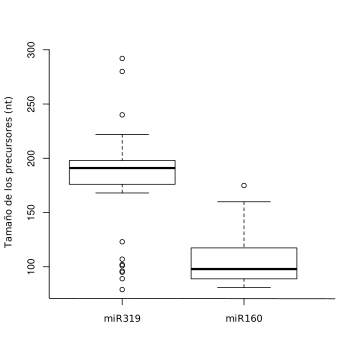
\includegraphics[width=.6\textwidth]{hairpin_distribution.png}
    \caption[Tamaño de precursores]{Tamaño de precursores. Se muestra el tamaño (nt) de dos familias de precursores en distintas especies.}
    \label{fig:hairpin_distribution}
\end{figure}

Además, en las plantas, las mutaciones que impiden la biogénesis o actividad de los miARNs, tales como \textit{hyl1}, \textit{hen1} y \textit{ago1}, conducen al aumento en los niveles de los transcriptos de muchos de los genes blanco de miARNs (aproximadamente un 45\% de todos los blancos) \citep{Han2004,pmid12747833,pmid16889646,Allen2005207}.
Esto sugiere que el mecanismo que involucra el corte y degradación de los ARNm es un componente importante de la represión inducida por los miARNs en plantas \citep{Jones-Rhoades2006, Voinnet2009669}.

En particular, la biogénesis de los miARNs es un proceso clave porque determina la secuencia exacta de nucleótidos del ARN pequeño funcional.
Si bien en el caso de animales está claro cuáles elementos estructurales son reconocidos en los precursores durante su procesamiento, poco se sabía sobre el reconocimiento de los precursores de plantas por la maquinaria de procesamiento.

\subsection{Construcción de bibliotecas de SPARE para estudios genómicos de biogénesis de miARNs en plantas}

En el marco de una colaboración con el grupo del Dr. Blake Meyers (Delaware,USA), el cual se especializa en secuenciación y análisis de ARN pequeños, nos propusimos entender cómo se procesan los precursores de miARNs en plantas. 
Colegas del laboratorio realizaron una estrategia para analizar sistemáticamente intermediarios de procesamiento de miARNs y caracterizar la biogénesis de la mayoría de los miARNs conservados presentes en \textit{A. thaliana} mediante técnicas de secuenciación de alto rendimiento, utilizando los equipos de última generación disponibles en Delaware (USA).
Esta técnica desarrollada en el laboratorio se conoce como SPARE \citep{Schapire2013} (del inglés Specific Parallel Amplification of RNA Ends).

La estrategia utilizada a partir de los datos de bibliotecas de SPARE se muestra en la Figura \ref{fig:GR_fig1C}.
 
\begin{figure}[htbp!] 
    \centering    
    \includegraphics[width=.3\textwidth]{GR_fig1C.png}
    \caption[Esquema del procedimiento para analizar los datos de SPARE]{
        \textbf{Esquema del procedimiento para analizar los datos de SPARE.}
    }
    \label{fig:GR_fig1C}
\end{figure}

Utilizando la técnica de SPARE se identifican los intermediarios de procesamiento de cada uno de los precursores de \textit{A. thaliana}, y uniendo la información brindada por los diferentes fragmentos es posible dilucidar tanto la dirección, como el número de cortes requeridos para la biogénesis de cada miARN (Figura \ref{fig:SPARE_tecnica}).
Es decir que no sólo se puede detectar la dirección de procesamiento, sino que también la técnica permite identificar precursores que requieren más de dos cortes para liberar el miARN maduro.

\begin{figure}[htbp!] 
	\centering    
	\includegraphics[width=1\textwidth]{SPARE_tecnica.png}
	\caption[Técnica de SPARE]{
        \textbf{Técnica de SPARE para diferenciar mecanismos de procesamiento de precursores.}
        Detalle donde se muestra a nivel molecular como la técnica permite diferenciar entre dos direcciones de procesamiento opuestas. 
    }
	 \label{fig:SPARE_tecnica}
\end{figure}

\subsection{Visualización de precursores que se procesan desde la base}

En el caso de los precursores que se procesan de base a loop, el único corte que puede ser detectado es el corte proximal (Figura \ref{fig:GR_fig2A}).

\begin{figure}[htbp!] 
    \centering    
    \includegraphics[width=.8\textwidth]{GR_fig2A.png}
    \caption[Identificación y caracterización de precursores de miARNs procesados de base a loop]{
    \textbf{Identificación y caracterización de precursores de miARNs procesados de base a loop.}
            Esquema donde se muestra la estructura secundaria del miR168a, miR172b y miR395b.
            Las flechas indican la posición y número de lecturas de los cortes del precursor identificado.
            Flechas en verde muestra el corte más abundante, que también coincide con al corte proximal del miARN/miARN*.
            Flechas en negro muestran otros cortes con al menos 5\% de abundancia del número total de cortes, mientras que otros cortes minoritarios se muestran con una flecha gris.
            Con rosa se resalta el stem de 15nt debajo del corte proximal.
            El miARN se indica en color rojo y el miARN* en color azul.
            La imagen de la derecha muestra el patrón de corte típico detectado en la biblioteca de SPARE para estos precursores.}
    \label{fig:GR_fig2A}
\end{figure}

\subsection{Visualización de precursores que se procesan desde el loop}

Para los precursores que se procesan de loop a base, la técnica de SPARE permite detectar tanto el corte distal como el proximal, que son los necesarios para liberar al miARN maduro.

\begin{figure}[htbp!] 
    \centering    
    \includegraphics[width=.8\textwidth]{GR_fig4A.png}
    \caption[Identificación y caracterización de precursores de miARNs procesados de loop a base]{
    \textbf{Identificación y caracterización de precursores de miARNs procesados de loop a base.}
    Esquema donde se muestra la estructura secundaria del miR156a, miR156c, miR156d y miR160a.
    Las flechas indican la posición y número de lecturas de los cortes del precursor identificado.
    Flechas en verde muestra el corte más abundante, que también coincide con al corte proximal del miARN/miARN*.
    Flechas en negro muestran otros cortes con al menos 5\% de abundancia del número total de cortes, mientras que otros cortes minoritarios se muestran con una flecha gris.
    Con gris se resalta el stem de arriba del miR156 y miR160. El miARN se indica en color rojo y el miARN* en color azul.
    La imagen de la derecha muestra el patrón de corte típico detectado en la biblioteca de SPARE para estos precursores.
}
    \label{fig:GR_fig4A}
\end{figure}


\section{Resultados y Discusión}

%~ \subsection{Procesamiento de precursores de miARNs en plantas}
%~ \label{sec:procesamiento}

\subsubsection{Desarrollo de herramienta para el análisis de intermediarios de procesamiento en plantas}

En una primera tanda de experimentos, Nicolás Bologna y Arnaldo Schapire realizaron bibliotecas de SPARE en Col-0 para estudiar los intermediarios de procesamiento en \textit{A. thaliana}.
De esta técnica, se obtienen una gran cantidad de datos para cada biblioteca secuenciada.
Estos datos se conocen como datos crudos y son fragmentos de secuencia que luego tienen que ser mapeados contra el genoma de datos de interés.
En este caso, el procesamiento de los datos crudos para obtener los datos finales lo realizaron en el laboratorio del Dr. Blake Meyers, que fue donde se realizaron las secuenciaciones.

%~ Además, estos datos crudos cuentan con información de las secuencia, lo que permite mediante programas informáticos hacer un control de calidad de la secuencias obtenidas.
%~ En total se obtuvieron cerca de 150 millones de secuencias (Figura \ref{fig:SPARE_estrategia}).

%~ Esos fragmentos son agrupados y mapeados contra las secuencias únicas de los precursores de \textit{A. thaliana}.
%~ Nos quedamos con 7158 secuencias únicas, que luego las filtramos por largo de la secuencia (Figura \ref{fig:SPARE_estrategia}).
%~ Esa información ya procesada es la que utilizamos en la herramienta para analizar y comparar los intermediarios de procesamiento para plantas silvestreste y mutantes de procesamiento.

%~ \begin{figure}[htbp!] 
	%~ \centering    
	%~ \includegraphics[width=.5\textwidth]{SPARE_estrategia.png}
	%~ \caption[Análisis informático utilizado para procesar los datos de SPARE]{
	%~ \textbf{Análisis informático utilizado para procesar los datos de SPARE.}
	%~ Las secuencias únicas mapeadas contra los precursores son las que se utilizan en la herramienta para analizar los intermediarios de procesamiento.
	%~ }
	 %~ \label{fig:SPARE_estrategia}
%~ \end{figure}

Para facilitar el análisis de los datos obtenidos por la técnica de SPARE, creamos una herramienta web disponible en la red interna del laboratorio.
La herramienta permite seleccionar un precursor en particular de los $\sim$100 precursores que se detectaron fragmentos por la técnica de SPARE.
Luego se selecciona una o varias mutantes y controles que se quieren analizar.
Además la herramienta permite modificar otros parámetros como la longitud y abundancia de los fragmentos secuenciados a considerar.

Primero vemos la salida de la herramienta para el precursor del  miR165a, analizando distintas mutantes de procesamiento al mismo tiempo (Figura \ref{fig:miR165a_SPARE}).
La posición final del duplex miARN/miARN* fue considerada como la posición 0, y las posiciones positivas son bases hacia arriba del dúplex mientrás que las posiciones negativas son bases hacia abajo del dúplex.
Los fragmentos se muestran en forma porcentual tomando cada biblioteca de forma independiente y en distintos colores se representan las distintas bibliotecas.
Además se muestra una tabla con los valores absolutos de cada fragmento y con flechas verdes se marcan las posiciones con los fragmentos de mayor abundancia en promedio de todas las bibliotecas (Figura \ref{fig:miR165a_SPARE}).
 
En esta figura se muestra un precursor que es procesado con un mecanismo corto de base a loop, donde según se muestra en la Figura \ref{fig:SPARE_tecnica}, los fragmentos detectados corresponden únicamente al primer corte por DCL1 (Figura \ref{fig:miR165a_SPARE}).
Se pueden observar también cortes en las posiciones $\pm 2$ con respecto a las esperadas por actividad "sloopy" (poco rigurosa) de DCL1 \citep{pmid17989254}.
Además se observan en la posición -5, que aparecen fragmentos en todas las bibliotecas aunque en muy baja abundancia (Figura \ref{fig:miR165a_SPARE}).

Mediante esta herramienta no sólo se puede identificar los precursores procesados de base a loop o de loop a base, sino que también permite identificar a los precursores que denominamos secuenciales, que son los que requieren de más de dos cortes por DCL1 para liberar al miARN maduro.
Por ejemplo, mostramos al precursor del miR169d que es procesado de forma secuencial de base a loop.
En estos precursores, los sitios de cortes delestán localizados 21 nt por debajo del lado proximal del dúplex miARN/miARN* y luego DCL1 sigue cortando para procesar al precursor.
En este caso se detecta un fragmento mayoritario en la posición -21, es decir 21nt por debajo del dúplex miARN/miARN* como era esperado para precursores secuenciales de base a loop \ref{fig:miR169d_SPARE}.

El precursor del miR169d tiene una estructura particular donde presenta un loop terminal ramificado.
Se ha estudiado este tipo de precursores, con esta estructura, donde se demostró que pueden ser procesados por DCl1 de manera bidireccional de base a loop o de loop a base, resultando en un procesamiento productivo y abortivo respectivamente \citep{pmid23934148}.
Con la herramienta desarrollada por nosotros, se puede observar que este precursor particular presenta fragmentos que provienen del corte secuencial de la base al loop que corresponde a la posición -21 en el gráfico.
Pero además, en la mutante de \textit{fiery} se pueden observar fragmentos que corresponden a un corte abortivo por DCL1 a partir del reconocimiento de este loop ramificado \ref{fig:miR169d_SPARE}.
La herramienta permite discriminar este tipo de procesamiento en distintas mutantes de procesamiento. 

\begin{landscape}
    \begin{figure}[htbp!] 
        \centering    
        \includegraphics[width=1.4\textwidth]{miR165a_SPARE.png}
        \caption[Captura de pantalla de la herramienta de SPARE para el miR165a]{
        \textbf{Captura de pantalla de la herramienta de SPARE para el miR165a.}
        Porcentaje de fragmentos del precursor (abundancia relativa de los fragmentos en esa posición dividido la abundancia total de los fragmentos en el precursor).
        La posición final del duplex miARN/miARN* fue considerada como la posición 0.
        La tabla muestra los valores absolutos de cada fragmento.
        Las flechas verdes marcan las posiciones del precursor con los fragmentos de mayor abundancia. 
        }
         \label{fig:miR165a_SPARE}
    \end{figure}
\end{landscape}

\begin{landscape}                                                                      
\begin{figure}[htbp!] 
        \centering    
        \includegraphics[width=1.4\textwidth]{miR169d_SPARE.png}
        \caption[Captura de pantalla de la herramienta de SPARE para el miR169d]{
        \textbf{Captura de pantalla de la herramienta de SPARE para el miR169d.}
        Porcentaje de fragmentos del precursor (abundancia relativa de los fragmentos eosición dividido la abundancia total de los fragmentos en el precursor).
        La posición final del duplex miARN/miARN* fue considerada como la posición 0.
        La tabla muestra los valores absolutos de cada fragmento.
        Las flechas verdes marcan las posiciones del precursor con los fragmentos de mayor abundancia. 
        }
	 \label{fig:miR169d_SPARE}
    \end{figure}
\end{landscape}

Para el caso de los precursores cortos de loop a base, los fragmentos detectados pueden ser más de uno según muestra la técnica de SPARE (Figura \ref{fig:SPARE_tecnica}).
Vemos el precursor del miR156a, donde los cortes más abundantes corresponden a las posiciones 22 y 0 (Figura \ref{fig:miR156a_SPARE}).
Estos fragmentos corresponden a los cortes del precursor por DCL1, donde el primer corte se da en la parte distal del dúplex y el segundo en la parte proximal del mismo.
Además se pueden observar otros fragmentos con abundancias relativas, cercanas a estas posiciones. 
En algunas bibliotecas se puede observar que acumulan más el primer corte (por ejemplo la biblioteca de Col\_AD) y en otras el segundo es el más abundate (biblioteca de Fiery\_1AB) (Figura \ref{fig:SPARE_tecnica}).
Esto podría ser interesante para estudiar en un futuro.
Además se puede observar que en \textit{Hyl} y \textit{Serrate} hay otros fragmentos con abundancia relativa en otras posiciones que las esperadas (posición 3 y posición 14 respectivamente), sugeriendo que tal vez que los cortes podrían estar afectados en estas mutantes de procesamiento (Figura \ref{fig:SPARE_tecnica}).

Por último en el caso del miR159, y al igual que todos los precursores que son procesados secuenciales de loop a base los cuatros fragmentos más abundantes corresponden a los cuatro cortes realizados por DCL1 que son requeridos para procesar este precursor (Figura \ref{fig:miR159b_SPARE}).
El primer corte se da en la posición 71, que de los cuatros cortes es el que tiene fragmentos menos abundantes, y luego DCL1 corta a 21 nucleótidos liberando otros ARN pequeños.
Luego se pueden observar los fragmentos correspondientes al tercer (posición 21) y cuarto corte (posición 0), que son los necesarios para liberar el miARN maduro (Figura \ref{fig:miR159b_SPARE}).
En este caso se pueden ver otros fragmentos que son productos de la degreadación del precursor, aunque nunca son tan abundantes como los fragmentos de los cortes por DCL1.
Por cuestiones de simplicidad, en la tabla solo se muestra los fragmentos con mayor abundancia en promedio de todas las bibliotecas.


\begin{landscape}
    \begin{figure}[htbp!] 
        \centering    
        \includegraphics[width=1.4\textwidth]{miR156a_SPARE.png}
        \caption[Captura de pantalla de la herramienta de SPARE para el miR156a]{
        \textbf{Captura de pantalla de la herramienta de SPARE para el miR156a.}
        Herramienta para analizar los datos de la técnica SPARE.
        Porcentaje de fragmentos del precursor (abundancia relativa de los fragmentos en esa posición dividido la abundancia total de los fragmentos en el precursor).
        La posición final del duplex miARN/miARN* fue considerada como la posición 0.
        La tabla muestra los valores absolutos de cada fragmento.
        Las flechas verdes marcan las posiciones del precursor con los fragmentos de mayor abundancia. 
        }
         \label{fig:miR156a_SPARE}
    \end{figure}
\end{landscape}



\begin{landscape}
    \begin{figure}[htbp!] 
        \centering    
        \includegraphics[width=1.4\textwidth]{miR159b_SPARE.png}
		\caption[Captura de pantalla de la herramienta de SPARE para el miR159b]{
        \textbf{Captura de pantalla de la herramienta de SPARE para el miR159b.}
        Porcentaje de fragmentos del precursor (abundancia relativa de los fragmentos en esa posición dividido la abundancia total de los fragmentos en el precursor).
        La posición final del duplex miARN/miARN* fue considerada como la posición 0.
        La tabla muestra los valores absolutos de cada fragmento.
        Por cuestiones de simplicidad, solo se muestran en la tabla los fragmentos con mayor abundancia en promedio de todas las bibliotecas.
        Las flechas verdes marcan las posiciones del precursor con los fragmentos de mayor abundancia.
        }
		\label{fig:miR159b_SPARE}
    \end{figure}
\end{landscape}



%~ -----------------------------------



%~ ################################################# 
%~ Identificación de intermediarios de procesamiento
%~ en plantas mutantes en proteínas de procesamiento
%~ #################################################

\subsection{Identificación de intermediarios de procesamiento en plantas mutantes en proteínas de procesamiento}

%~ La técnica de SPARE (del inglés Specific Parallel Analisys of 5'RNA Ends) fue desarrollada con el objetivo de caracterizar el procesamiento de los precursores de miARNs de \textit{A. thaliana}.
%~ Para esto se identifican los intermediarios de procesamiento de cada uno de dichos precursores, y uniendo la información brindada por los diferentes fragmentos es posible dilucidar tanto la dirección, como el número de cortes requeridos para la biogénesis de cada miARN (Figura \ref{fig:SPARE_tecnica}).

%~ \begin{figure}[htbp!] 
	%~ \centering    
	%~ \includegraphics[width=1\textwidth]{SPARE_tecnica.png}
	%~ \caption[Técnica de SPARE]{
        %~ \textbf{Técnica de SPARE para diferenciar mecanismos de procesamiento de precursores.}
        %~ Detalle donde se muestra a nivel molecular como la técnica permite diferenciar entre dos direcciones de procesamiento opuestas. 
    %~ }
	 %~ \label{fig:SPARE_tecnica}
%~ \end{figure}

%~ Brevemente la técnica consiste en emplear los extremos 5'P dejados por la maquinaria de procesamiento en los precursores luego del clivaje para realizar una ligación ARN-ARN entre los intermediaros de procesamiento y un oligo de ARN de secuencia conocida.
%~ A continuación se emplean oligos específicos para retro-transcribir los intermediaros de cada precursor en particular, con una cola común a todos.
%~ En este punto todos los fragmentos generados durante el procesamiento presentan los mismos extremos: en el 5' la secuencia del oligo de ARN y el en el extremo 3' la secuencia común incorporada durante la retro-transcripción.
%~ Esta información es empleada para diseñar oligos (FW y RV) que se emplean en una reacción de PCR a continuación.
%~ Finalmente los fragmentos son secuenciados. 

En la sección \ref{sec:procesamiento} mostramos los resultados obtenidos de esta técnica para determinar la dirección de procesamiento de los precursores de miARNs en plantas.
Esta nueva secuenciación se realizó debido que anteriormente no se pudieron de determinar la dirección de procesamiento de algunos precursores.
Además, en esta nueva tanda de secuenciación de precursores se intentó identificar intermediarios de procesamiento en plantas mutantes en proteínas de procesamiento.  
Para esta parte del trabajo se hicieron algunas modificiaciones de la técnica.
Se ubicaron los oligos a 100 nt del último corte 3' esperado.
En total se diseñaron 121 oligos para retrotranscribir el conjunto de precursores conservados y jóvenes validados hasta el momento.  
Además, anteriormente el procesamiento de los datos a partir de los datos crudos se hicieron en el mismo laboratorio que se realizaron las secuenciaciones.

\subsubsection{Construcción de bibliotecas multiplex}
El paso final consiste en secuenciar las bibliotecas construidas, sin embargo la secuenciación es costosa haciendo económicamente dificultoso secuenciar varias bibliotecas en paralelo para comparar entre diferentes condiciones (siendo este nuestro objetivo con las plantas mutantes en proteínas de procesamiento).
En los últimos años se han desarrollado métodos que hacen posible secuenciar más de una biblioteca por calle.
Esto consiste en marcar los fragmentos provenientes de cada biblioteca con secuencias especificas (detallado en Materiales y Métodos) y separar informáticamente cada secuencia en la biblioteca de la cual provino a luego de secuenciación.
Técnicamente esto se hace agregando una PCR final donde los índex son incorporados en todas las secuencias de cada biblioteca.

\subsubsection{Diseño experimental}

Con el objetivo de construir bibliotecas de SPARE crecimos plántulas de Arabidopsis thaliana durante 10 días con luz continúa (independizándonos de este modo la variación asociada al ritmo circadiano a la hora de la colecta de muestra).
Se realizó un experimento con plantas mutantes en proteínas de procesamiento.

\textbf{Plantas mutantes en proteínas de procesamiento}

\textit{Hyl1}, \textit{Se} y \textit{Fiery}.
Siendo sus controles plantas silvestres de Arabidopsis ecotipo Col-O.

%~ \textbf{Plantas sometidas a diferentes temperaturas}
%~ 
%~ En este caso sólo se utilizaron plantas Col-0 y fiery crecidas en las condiciones descriptas anteriormente y que luego fueron sometidas a un tratamiento de dos horas a tres temperaturas diferentes: 8 \degree C, 22 \degree C y 37 \degree C.
%~ Luego se realizó la colecta de muestra a la temperatura del tratamiento. 



%~ ESTO VA EN LA PARTE 2 DE RESULTADOS!!!!!!!!!!
%~ Para ver si había diferencias estructurales para los precursores con diferentes mecanismos de procesamiento, determinamos la estructura secundaria de precursores detectados que se procesan en dirección base a loop (Figura \ref{fig:GR_fig2C}) y los que se procesan loop a base (Figura \ref{fig:GR_fig4C}).
%~ Obtuvimos las estructuras secundarias para cada precursor.
%~ Definimos a una coincidencia en cada posición con un 0, mientras que "bulges" y "mismatches" los consideramos como 1.
%~ El lado proximal del duplex miARN/miARN* fue definido como la posición +1 y analizamos desde la posición -25 a la posición +40 (Figura \ref{fig:GR_fig2C} y \ref{fig:GR_fig4C}). 

%~ -------- Esto en la conclusion
%~ Utilizando esta técnica encontramos que los miARNs son procesados por cuatro mecanismos, dependientes de la dirección secuencial de la maquinaria de procesamiento y del número de cortes requeridos para liberar el miARN.
%~ La clasificación de los precursores, teniendo en cuenta los mecanismos de procesamiento, reveló determinantes estructurales específicos para cada grupo.
%~ Se encontró que la complejidad de las vías de procesamiento de miARN se produce tanto en precursores jóvenes como en conservados y que los miembros de la misma familia pueden ser procesados de diferentes maneras.
%~ Además hemos observado que diferentes determinantes estructurales compiten por la maquinaria de procesamiento y que miARNs alternativos pueden ser generados a partir de un único precursor.
%~ Los resultados ofrecen una explicación para la diversidad estructural de los genes de precursores de miARN en plantas y nuevas perspectivas hacia la comprensión de la biogénesis de los ARNs pequeños \citep{Bologna2013}.


%~ Esto no se si va a algun lado
%~ Mediante la cantidad de cortes detectados la técnica de SPARE permite definir si el mecanismo es base a loop o loop a base.
%~ Esta técnica arroja una gran cantidad de datos producto de la secuenciación de alto rendimiento, por lo que se necesita de un enfoque bioinformático para la interpretación de los resultados.
%~ Por la gran cantidad de precursores a estudiar y el número de bibliotecas se necesitó un análisis previo de los datos y una forma de presentarlos.
%~ Para esto construimos e implementamos un pipeline bioinformático utilizando "in-house" scripts y datos disponibles de miRBASE para poder analizar los datos de las bibliotecas de deep-sequencing obtenidos a partir de la técnica de SPARE.
%~ Un precursor fue considerado como detectado si más de tres lecturas corresponden a la secuencia de ese precursor.
%~ De esta manera encontramos fragmentos de ARN que corresponden a 129 precursores, 71 de ellos de miARNs conservados y 58 de miARNs jóvenes (Figura \ref{fig:GR_fig1C}).
%~ Mediante el análisis de los datos arrojados de la estrategia bioinformática pudimos definir la dirección de procesamiento de la mayoría de los precursores en \textit{A. thaliana}.
%~ De los cuales 32 de ellos fueron definidos como procesados por un mecanismo de base a loop, ya que se encontraron los cortes en la parte proximal del duplex miARN/miARN* sin detectar cortes en la parte de arriba del duplex, como en el caso del miR168a, miR172b y el miR395b (Figura \ref{fig:GR_fig2A}).
%~ Además encontramos 16 precursores de miARNs conservados con cortes detectados (>5\%) en el lado distal del miARN/miARN* los cuales fueron definidos como loop a base (Figura \ref{fig:GR_fig4A}).

%~ # Esto va al final, pueden ir los dos juntos
%~ \subsection{Visualización de precursores que se procesan desde la base}
%~ Consideramos la estructura secundaria de 32 precursores analizados en esta parte del trabajo que se procesan de base a loop y todos ellos tienen un claro tallo inferior de 15 nt de largo (Figura \ref{fig:GR_fig2C}).
%~ Además este tallo se pudo ver tanto para los precursores validados experimentalmente que se procesan de base a loop como para todos los precursores conservados (Figura \ref{fig:GR_fig2C} en violeta).
%~ Pero pudimos observar que las bases inmediatamente debajo del duplex miARN/miARN* (posición -2 y -1) tienden a estar desapareadas (Figura \ref{fig:GR_fig2C}).
%~ Además las posiciones -3 y -4 y las 3 últimas posiciones del stem inferior (-13,-14 y -15) están apareadas casi siempre (Figura \ref{fig:GR_fig2C}).
%~ En general, nuestros resultados muestran que los precursores procesados en una dirección base a loop son más uniformes de lo que se pensaba previamente y que al menos algunos de los precursores no detectados como base a loop probablemente tengan otros determinantes específicos de ARN.
%~ 
%~ \subsection{Visualización de precursores que se procesan desde el loop}
%~ Estos precursores, que tienen un procesamiento loop a base, tienen un corte mayoritario que se puede detectar en nuestras bibliotecas.
%~ Este corte es el esperado en la dirección de procesamiento de precursores con un mecanismo de loop a base.
%~ Con la excepción de dos miARNs (miR396a y miR162b) estos precursores no tienen una estructura obvia debajo del duplex miARN/miARN* (Figura \ref{fig:GR_fig4C}).
%~ Estos precursores tienen una región terminal estructurada (Figura \ref{fig:GR_fig4C}), que tiene un tamaño homogéneo de ~42nt que incluye un loop corto en contraste con la misma región en los precursores que se procesan de base a loop donde es más variable (Figura \ref{fig:GR_fig2C} y \ref{fig:GR_fig4C}). 


%~ \begin{figure}[htbp!] 
    %~ \centering    
    %~ \includegraphics[width=1\textwidth]{GR_fig2C.png}
    %~ \caption[Estructura secundaria de precursores de base a loop]{Estructura secundaria de precursores detectados que se procesan en dirección base a loop.
    %~ Los matches en cada posición los consideramos como 0, mientras que "bulges" y "mismatches" fueron considerados como 1.
    %~ La estructura secundaria considerando todos los miARNs conservados se indica con color violeta.
    %~ }
    %~ \label{fig:GR_fig2C}
%~ \end{figure}
%~ 
%~ \begin{figure}[htbp!] 
    %~ \centering    
    %~ \includegraphics[width=1\textwidth]{GR_fig4C.png}
    %~ \caption[Estructura secundaria de precursores de loop a base]{
    %~ Estructura secundaria de precursores detectados que se procesan en dirección loop a base.
    %~ Los matches en cada posición los consideramos como 0, mientras que "bulges" y "mismatches" fueron considerados como 1.}
    %~ \label{fig:GR_fig4C}
%~ \end{figure}


%~ ######## ESTO PUEDE IR AL FINAL FINAL
%~ En esta segunda parte del proyecto de tesis presentamos un estrategia y realizamos un análisis sistemático para la identificación de la biogénesis de precursores de miARNs desde un punto de vista genómico.
%~ De esta manera pudimos encontrar la dirección de procesamiento de la mayoría de los precursores de miARNs en \textit{A. thaliana}.
%~ Estos resultados fueron publicado en la revista Genome Research \citep{Bologna2013}.
%~ En este mismo artículo se pudo demostrar que los precursores de miARNs en plantas, se pueden agrupar por cuatro mecanismos de procesamiento con distintas características (Figura \ref{fig:mecanismos}).
%~ 
%~ \begin{itemize}
    %~ \item En los precursores con un mecanismo \textbf{corto de base a loop}, un loop interno seguido por un tallo inferior de $\sim$15nt especifica la posición del primer corte.
        %~ Esta estructura se encuentra en la mayoría de familias de miARNs \citep{Mateos2010,pmid20015653,pmid20015654}.
        %~ A pesar de que el tallo puede contener bulges, la transición de un loop interno (simple hebra) al tallo inferior es bastante marcada, y tres pares de bases apareadas generalmente definen el comienzo del tallo inferior del precursor \citep{Bologna2013}.
        %~ El segundo corte procede a una distancia fija de $\sim$21 nt desde la posición del primer corte.
    %~ \item En los precursores con un mecanismo \textbf{secuencial de base a loop} (ej: familia del miR169), el primer corte procede como en los cortos de base a loop, pero luego son necesario dos cortes más para liberar el miARN, generando en el proceso niveles bajos de RNA pequeños adicionales \citep{Bologna2013}.
    %~ \item En los precursores con un mecanismo \textbf{cortos de loop a base} (ej: familia del miR156 y miR160), el procesamiento es guiado por un tallo superior, y son necesarios dos cortes para liberar el miARN maduro.
        %~ La región terminal de estos precursores tienen una largo conservado de $\sim$42 donde incluye un loop pequeño \citep{Bologna2013}.
    %~ \item En los precursores con un mecanismo \textbf{secuencial de loop a base} (ej: familia del miR319 y miR159), cuatro cortes secuenciales por DCL1 son los encargados de procesar los precursores de miARNs.
        %~ En general muestran un tallo largo superior, del cual otros ARNs pequeños son generados \citep{pmid19850910,Bologna2009,Bologna2013}
%~ \end{itemize}
%~ 
%~ \begin{figure}[htbp!] 
    %~ \centering    
    %~ \includegraphics[width=1\textwidth]{mecanismos.png}
    %~ \caption[Mecanismos de procesamiento]{Distintos mecanismos de procesamientos de miARNs en plantas}
    %~ \label{fig:mecanismos}
%~ \end{figure}



\lhead{Capítulo 3}
%*******************************************************************************
%****************************** Second Chapter *********************************
%*******************************************************************************
\graphicspath{{Chapter3/Figs/}}

\setcounter{chapter}{6}
\chapter*{Resultados y Discusión Capítulo 3} 
\addcontentsline{toc}{chapter}{Resultados y Discusión Capítulo 3}

{\LARGE Estudios de la evolución y biogénesis de miARNs}


\section{Introducción}


\section{Resultados y Discusión}

%~ ################################################# 
%~ Enfoque bioinformático para el estudio de la
%~ evolución y biogénesis de miARNs en plantas
%~ #################################################

\subsection{Enfoque bioinformático para el estudio de la evolución y biogénesis de miARNs en plantas}

Que los precursores de miARNs en plantas sean procesados de diferentes maneras \citep{Bologna2013}, nos llevó a especular que su patrón de evolución también puede ser diferente y podrían estar vinculados a su mecanismo de procesamiento.
Es por esto que elaboramos una estrategia bioinformática para caracterizar la relación entre la evolución de los precursores de miARNs en plantas y los mecanismos de procesamiento determinados previamente.

\subsubsection{Estrategia}

La metodología utilizada se detalla en la sección \ref{ref_evolution} y primero la utilizamos para estudiar precursores de miARNs conservados en dicotiledóneas. 
La misma consta de los siguientes pasos:

\begin{itemize}
    \item Búsqueda de ortólogos para cada miembro de cada familia de Arabidopsis de  precursores de miARNs conservados en plantas
    \item Extensión de las secuencias
    \item Alineamiento de secuencia primaria
    \item Alineamiento de secuencia teniendo en cuenta estructura secundaria
    \item Búsqueda de motivos conservados
    \item Representación gráfica de los precursores
\end{itemize}

\subsubsection{Búsqueda de ortólogos de precursores de miARNs}

Las secuencias de los precursores de miARNs en miRBASE rara vez son validadas experimentalmente, de hecho muchas de ellas son el resultado de predicciones computacionales de estructuras en forma de tallo y burbuja que incluye el miARN maduro, pero que no se extiende muchas bases más allá de el mismo \cite{Kozomara2014}.
Esto lleva a anotaciones erróneas de los precursores de miARNs.
Además para cada miembro de cada familia de \textit{A. thaliana} no es trivial asignarle un ortólogo en otra especie teniendo en cuenta la anotación de miRBASE.

Por esto, primero realizamos una búsqueda de ortólogos para cada miembro de cada familia de \textit{A. thaliana} y empezamos nuestro análisis con una definición arbitraria de los precursores de plantas incluyendo 150 nt fuera del par miARN/miARN*.
Para la búsqueda de ortólogos, extensión de la secuencia y el posterior análisis de los precursores, utilizamos datos genómicos de plantas extraídos de Phytozome. 

Para la mayoría de los miembros de cada familia de precursores pudimos detectar ortólogos en otras especies. 
Teniendo en cuenta las 30 dicotiledóneas utilizadas en este estudio, en promedio, se encontraron ortólogos para cerca de 20 especies para cada precursor de miARN de \textit{A. thaliana} (Figura \ref{fig:dicots_species}).

\begin{figure}[htbp!] 
    \centering    
    
\includegraphics[width=.5\textwidth]{dicots_species.png}
    \caption[Especies detectadas]{Cantidad de especies detectadas.
    Esta figura muestra la distribución de la cantidad de especies donde se encuentran ortólogos de precursores de miARNs.
    A la izquierda se muestra la distribución de especies por miembro de familias de precursores de miARNs donde se detecta el ortólogo de \textit{A. thaliana}.
    A la derecha se agruparon todos los miembros de una misma familia y se muestra la distribución de la cantidad de especies donde se detecta un ortólogo de \textit{A. thaliana}}
    \label{fig:dicots_species}
\end{figure}

Algunos familias de miARNs se han diversificado durante la evolución, donde en algunas especies un miARN puede encontrarse como un único gen y en otras especie el mismo miARN puede encontrarse en múltiples miembros.
Por ejemplo, el miR396 en Arabidopsis está constituido por dos miembros, miR396a y miR396b mientras que en en el caso de arroz existen 8 miembros, nombrados del miR396a al miR396h.
Por esto, agrupamos a los miembros por familias y vimos la distribución de la cantidad de especies donde se detecta un ortólogo de los precursores de miARNs pertenecientes a \textit{A. thaliana} y en este caso vimos un alto número de especies detectadas para la mayoría de las familias de miARNs (Figura \ref{fig:dicots_species}).

\subsubsection{Alineamiento de los precursores en base a su secuencia primaria}

Comenzamos con los alineamientos múltiple de cada miembro de las familias de precursores de miARNs conservadas en dicotiledóneas.
Primero, realizamos el alineamiento en base a su secuencia primaria utilizando la herramienta T-Coffee \citep{pmid10964570}.
En la Figura \ref{fig:miR172a_tcoffee} se muestra el alineamiento del precursor del miR172a en distintas especies coloreado en base a la conservación evolutiva de la secuencia primaria.
Se puede observar que el miR172a maduro y el miR172a* están muy conservados en las distintas especies, pero además se puede ver una cola de conservación que podría corresponder al tallo inferior del precusor (Figura \ref{fig:miR172a_tcoffee}).

\begin{landscape}
    \begin{figure}[htbp!] 
        \centering    
        \includegraphics[width=1.4\textwidth]{miR172a_tcoffee.png}
        \caption[Alineamiento del precursor del miR172a.]{Alineamiento del precursor del miR172a. 
        Se muestra el alineamiento del precursor del miR172a en distintas especies. 
        En colores se muestra la conservación de la secuencia primaria, donde azul más oscuro denota mayor conservación y naranja menor conservación.
        Se muestran $\sim$60 bases por debajo del dúplex miARN/miARN* y los alineamientos están separados en dos líneas para una mejor representación.}
         \label{fig:miR172a_tcoffee}
    \end{figure}
\end{landscape}

Para poder corroborar esto y obtener información adicional sobre la conservación de los precursores, realizamos la predicción de estructura secundaria utilizando la herramienta RNAfold \citep{pmid22115189} (Figura \ref{fig:miR172a_rnafold}).
Además realizamos nuevamente los alineamientos pero considerando la estructura secundaria de los precursores, utilizando la herramienta R-Coffee \citep{pmid18292307}.

En la Figura \ref{fig:miR172a_rnafold} se puede observar que existe un patrón que comparten los precursores en la región debajo del miARN/miARN*.
No es simple reconocer patrones similares mirando los precursores de esta manera.
Además la cantidad de precursores estudiados en esta parte del trabajo de Tesis dificulta aún más este tipo de análisis.

\begin{landscape}
    \begin{figure}[htbp!] 
        \centering    
        \includegraphics[width=1.4\textwidth]{miR172a_rnafold.png}
        \caption[Estructura secundaria del miR172a en distintas especies]{
        Estructura secundaria del miR172a en distintas especies.
        Se muestra la estructura secundaria de los precursores del miR172a en distintas especies, calculados con la herramienta RNAfold.
        }
        \label{fig:miR172a_rnafold}
    \end{figure}
\end{landscape}

Para poder reconocer fácilmente la región conservada dentro del precursor y poder analizar más en detalle estos patrones de conservación, decidimos agrupar toda esta información
 generada a partir de los alineamientos de secuencia primaria y estructura secundaria en un gráfico circular como se muestra en la figura \ref{fig:miR172a_circos}.
Estos gráficos se hicieron utilizando el paquete Circos \citep{pmid19541911}.
 
En dicha figura se muestra el Circos del miR172a a modo de ejemplo.
Para representar el precursor, se tomaron 60 nt por debajo del dúplex miARN/miARN*.
En el anillo exterior se representa en colores el grado de conservación de la secuencia consenso a partir de los alineamientos en base a su secuencia primaria.
Además se muestran las bases del precursor de \textit {A. thaliana}.
Luego en el anillo interior se representa, mediante un histograma, la frecuencia de bases apareadas y desapareadas para cada posición del precursor en las distintas especies.
Con líneas de distinto espesor se muestra la interacción de las bases del precursor considerando la estructura secundaria. 
Fuera del anillo exterior se marca la secuencia del miARN y miARN*.

Realizamos los Circos para visualizar de manera simple los precursores de miARNs en distintas especies de plantas.
Y los utilizamos para caracterizar la relación entre los patrones de conservación y los mecanismos de procesamiento determinados previamente.


\begin{figure}[htbp!] 
    \centering    
    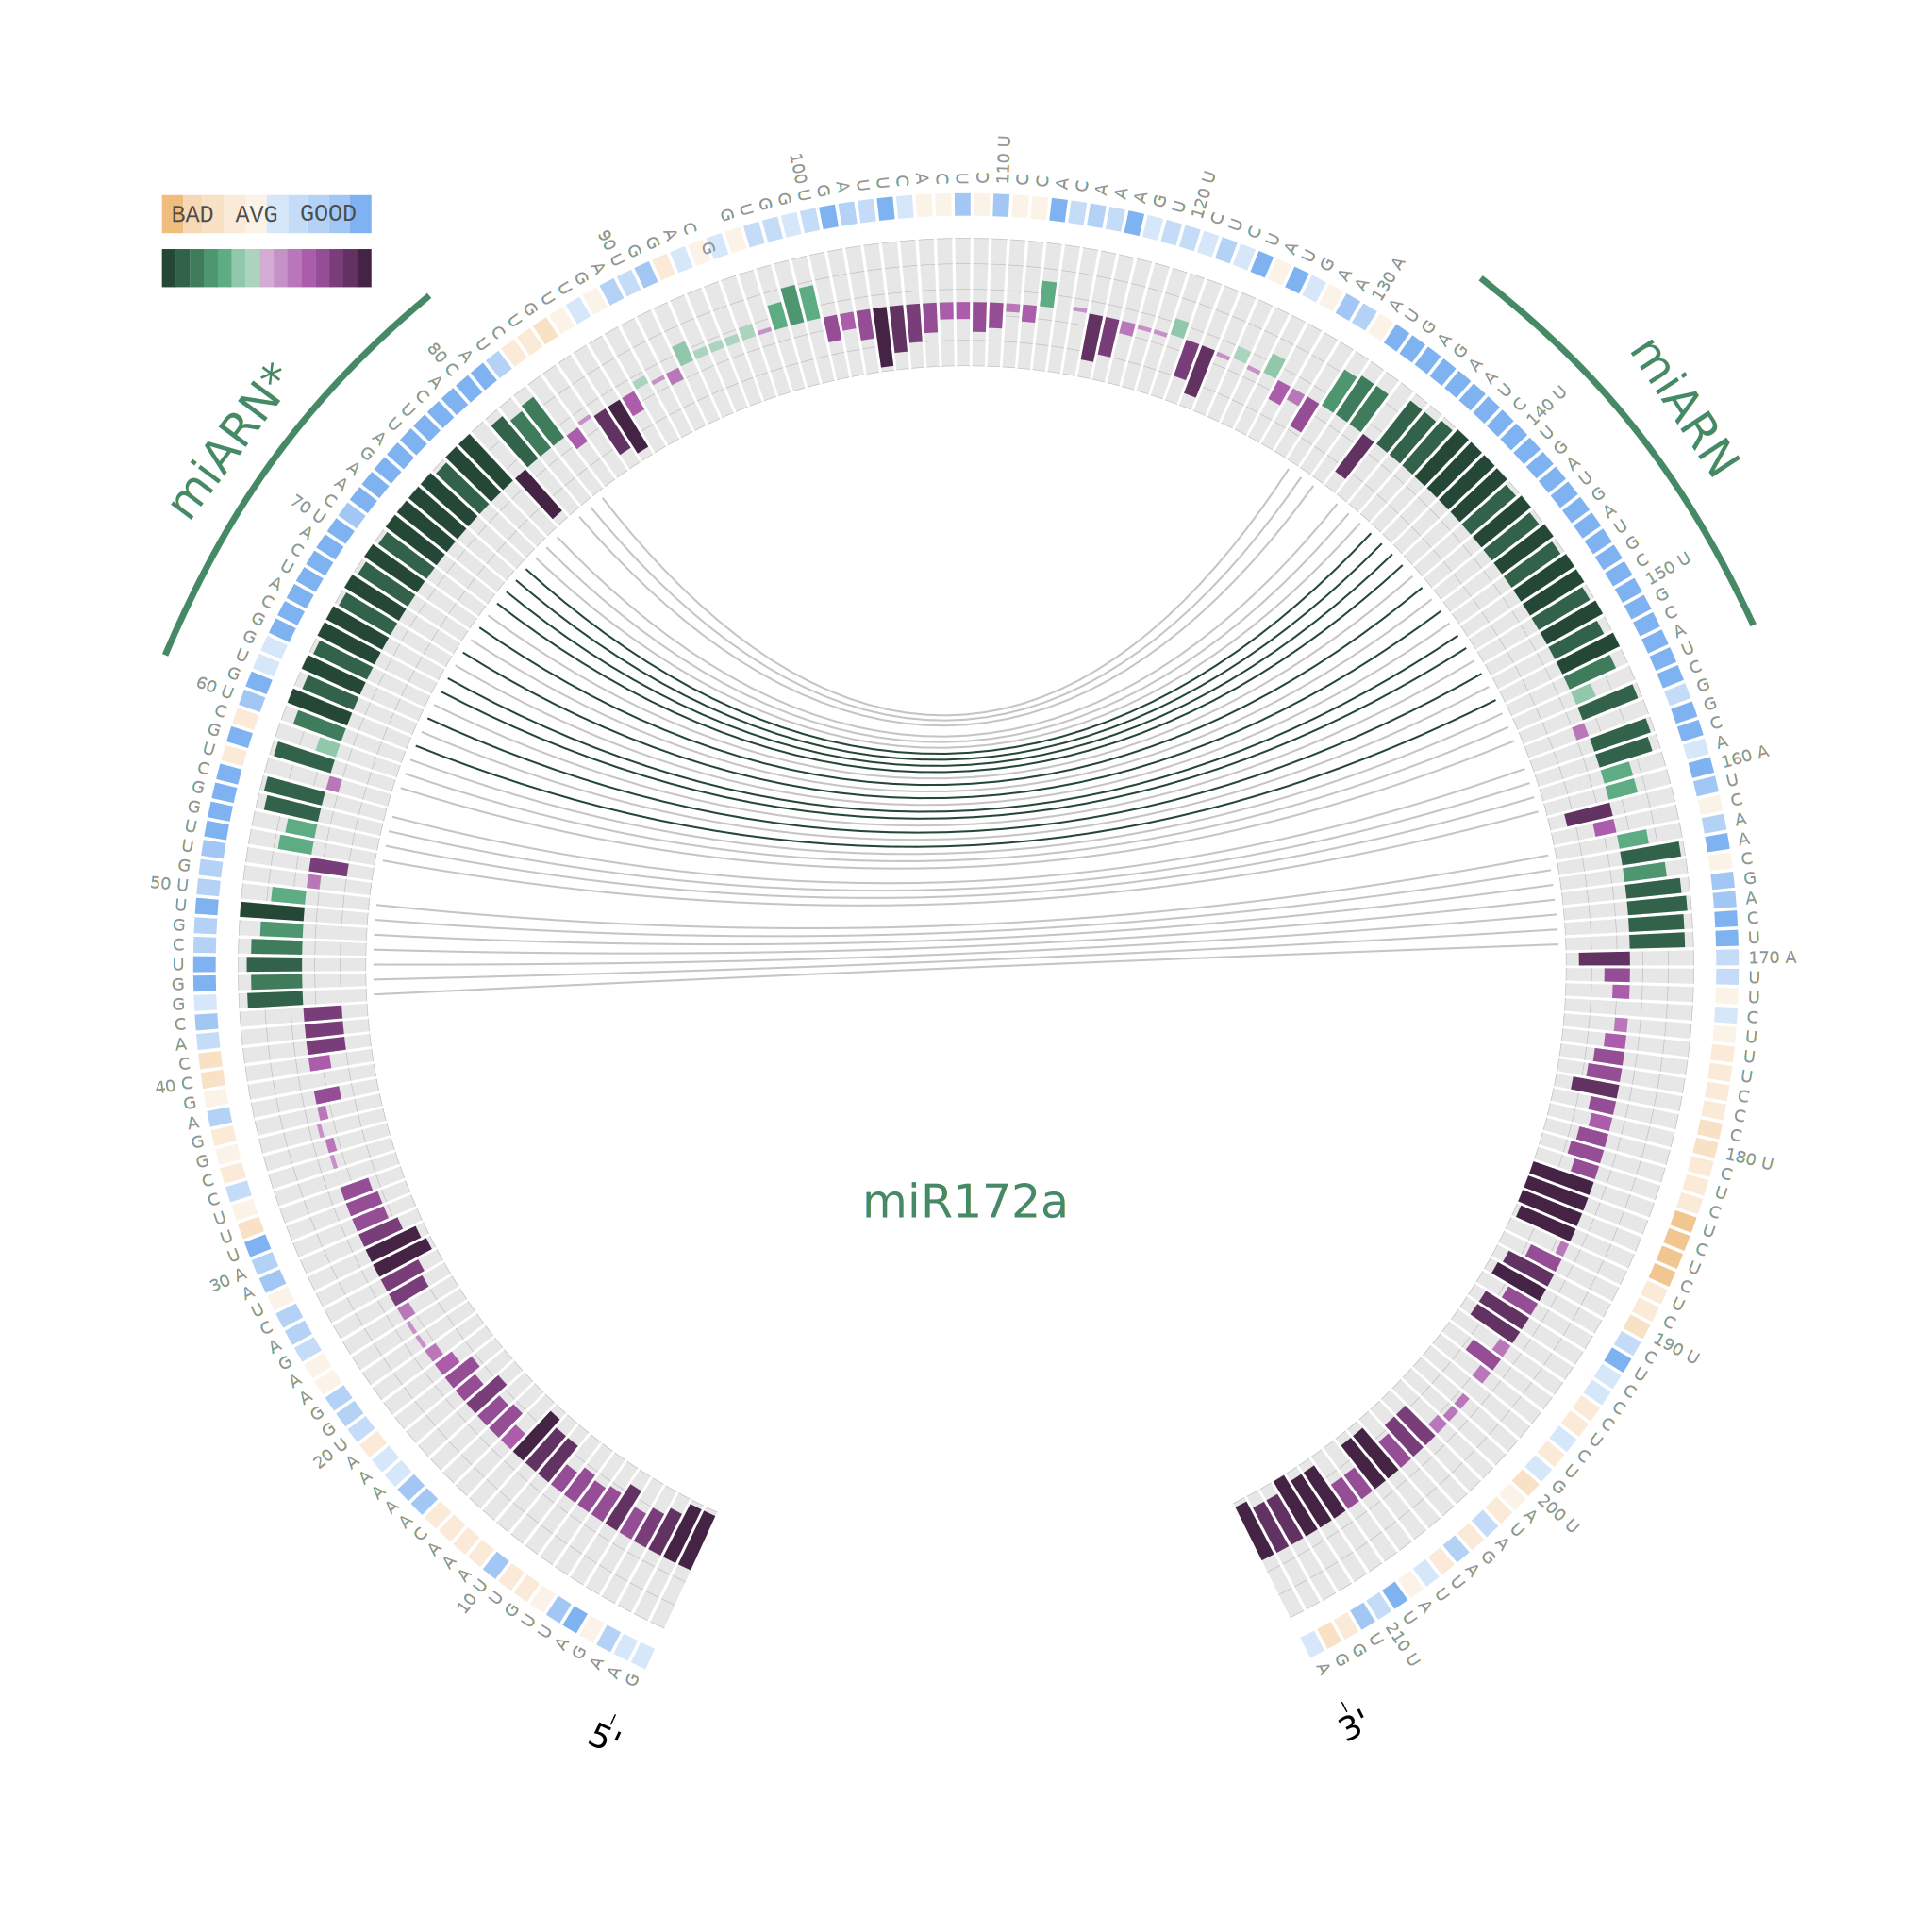
\includegraphics[width=1\textwidth]{miR172a_circos.png}
    \caption[Circos del miR172a]{Circos del miR172a.
En el anillo exterior se representa en colores el grado de conservación de la secuencia consenso a partir de los alineamientos en base a su secuencia primaria.
Además se muestran las bases del precursor de \textit {A. thaliana}.
Luego en el anillo interior se representa, mediante un histograma, la frecuencia de bases apareadas y desapareadas para cada posición del precursor en las distintas especies.
Con líneas de distinto espesor se muestra la interacción de las bases del precursor considerando la estructura secundaria. 
Fuera del anillo exterior se marca la secuencia del miARN y miARN*.
   }
     \label{fig:miR172a_circos}
\end{figure}

Por último, para cada precursor en distintas especies, realizamos una búsqueda de motivos conservados con la herramienta MEME \citep{pmid22115189} (Figura \ref{fig:miR172_meme}).
Hicimos esto para poder ver de manera visual cuáles eran los patrones comunes entre las distintas especies y donde se localizaban dentro del precursor.
Esta búsqueda de motivos la hicimos de diferentes maneras, la primera permitiendo encontrar hasta 2 motivos conservados en los precursores de distintas especies.


\begin{landscape}
    \begin{figure}[htbp!] 
        \centering    
        \includegraphics[width=1.4\textwidth]{miR172_meme.png}
        \caption[MEME del miR172a]{
			\textbf{MEME del miR172a.}
        Se muestra el MEME donde se pueden observar los motivos conservados dentro de los precursores del miR172a en distintas especies.
        En color rojo el primer motivo conservado comprende parte del miR172 (logo 1).
        El segundo motivo más conservado comprende parte del miR172* (logo 2).
        }
        \label{fig:miR172_meme}
    \end{figure}
\end{landscape}

\subsubsection{Mecanismo de base a loop cortos}

En los precursores con un mecanismo corto de base a loop, un loop interno seguido por un tallo inferior de $\sim$15nt especifica la posición del primer corte.
A pesar de que el tallo puede contener bulges, la transición de un loop interno (simple hebra) al tallo inferior es bastante marcada, y tres pares de bases apareadas generalmente definen el comienzo del tallo inferior del precursor \citep{Mateos2010,Bologna2013}.
El segundo corte procede a una distancia fija de $\sim$21 nt desde la posición del primer corte.

Para la mayoría de los precursores procesados con este mecanismo pudimos observar el mismo patrón de conservación de estructura primaria y similares patrones de estructura secundaria.
Para los precursores del miR172a (Figura \ref{fig:miR172a_circos} y el miR390a \ref{fig:miR390a_circos}), mediante la estrategia pudimos encontrar precursores en las 30 especies utilizadas.
En ambos casos, se pudo observar que la región con mayor conservación conincide con el duplex miARN/miARN* pero además se puede ver una región conservada por debajo del dúplex, que coincide con el tallo inferior.

Otra ventaja de esta forma de representar a los precursores con la conservación entre especies, es que visualmente se puede reconocer facilmente las posiciones donde existen "mismatches" conservados. 
Por ejemplo en el Circos del miR172, se puede observar un mismatch en la primer posición del miARN con la posición 19 del miARN*.
Esta interacción es A-A y se mantiene sin variaciones en todas las especies (Figura \ref{fig:miR172a_circos}).
Esto podría ser interesante estudiarlo en detalle donde se podría generar un precursor mutante donde esas bases en particular estén apareadas y luego ver si esto afecto o no el procesamiento del precursor.  
Además notamos que este patrón de conservación se puede observar independientemente si el miARN maduro está en la hebra 5' (Figura \ref{fig:miR172a_circos}) o si está en la hebra 3' (Figura \ref{fig:miR390a_circos}).

A diferencia de los precursores que tienen un mecanismo de loop a base, donde el tallo superior es fundamental para el su procesamiento, los precursores que se procesan cortos de base a loop no tienen el tallo superior conservado.
Y mediante la búsqueda de motivos conservados, pudimos observar que el tamaño del tallo superior y del loop es muy variado en un mismo precursor en distintas especies, donde los mismos puede ir desde los 40nt hasta 115nt (Figura \ref{fig:miR172_meme}).


\begin{figure}[htbp!] 
    \centering    
    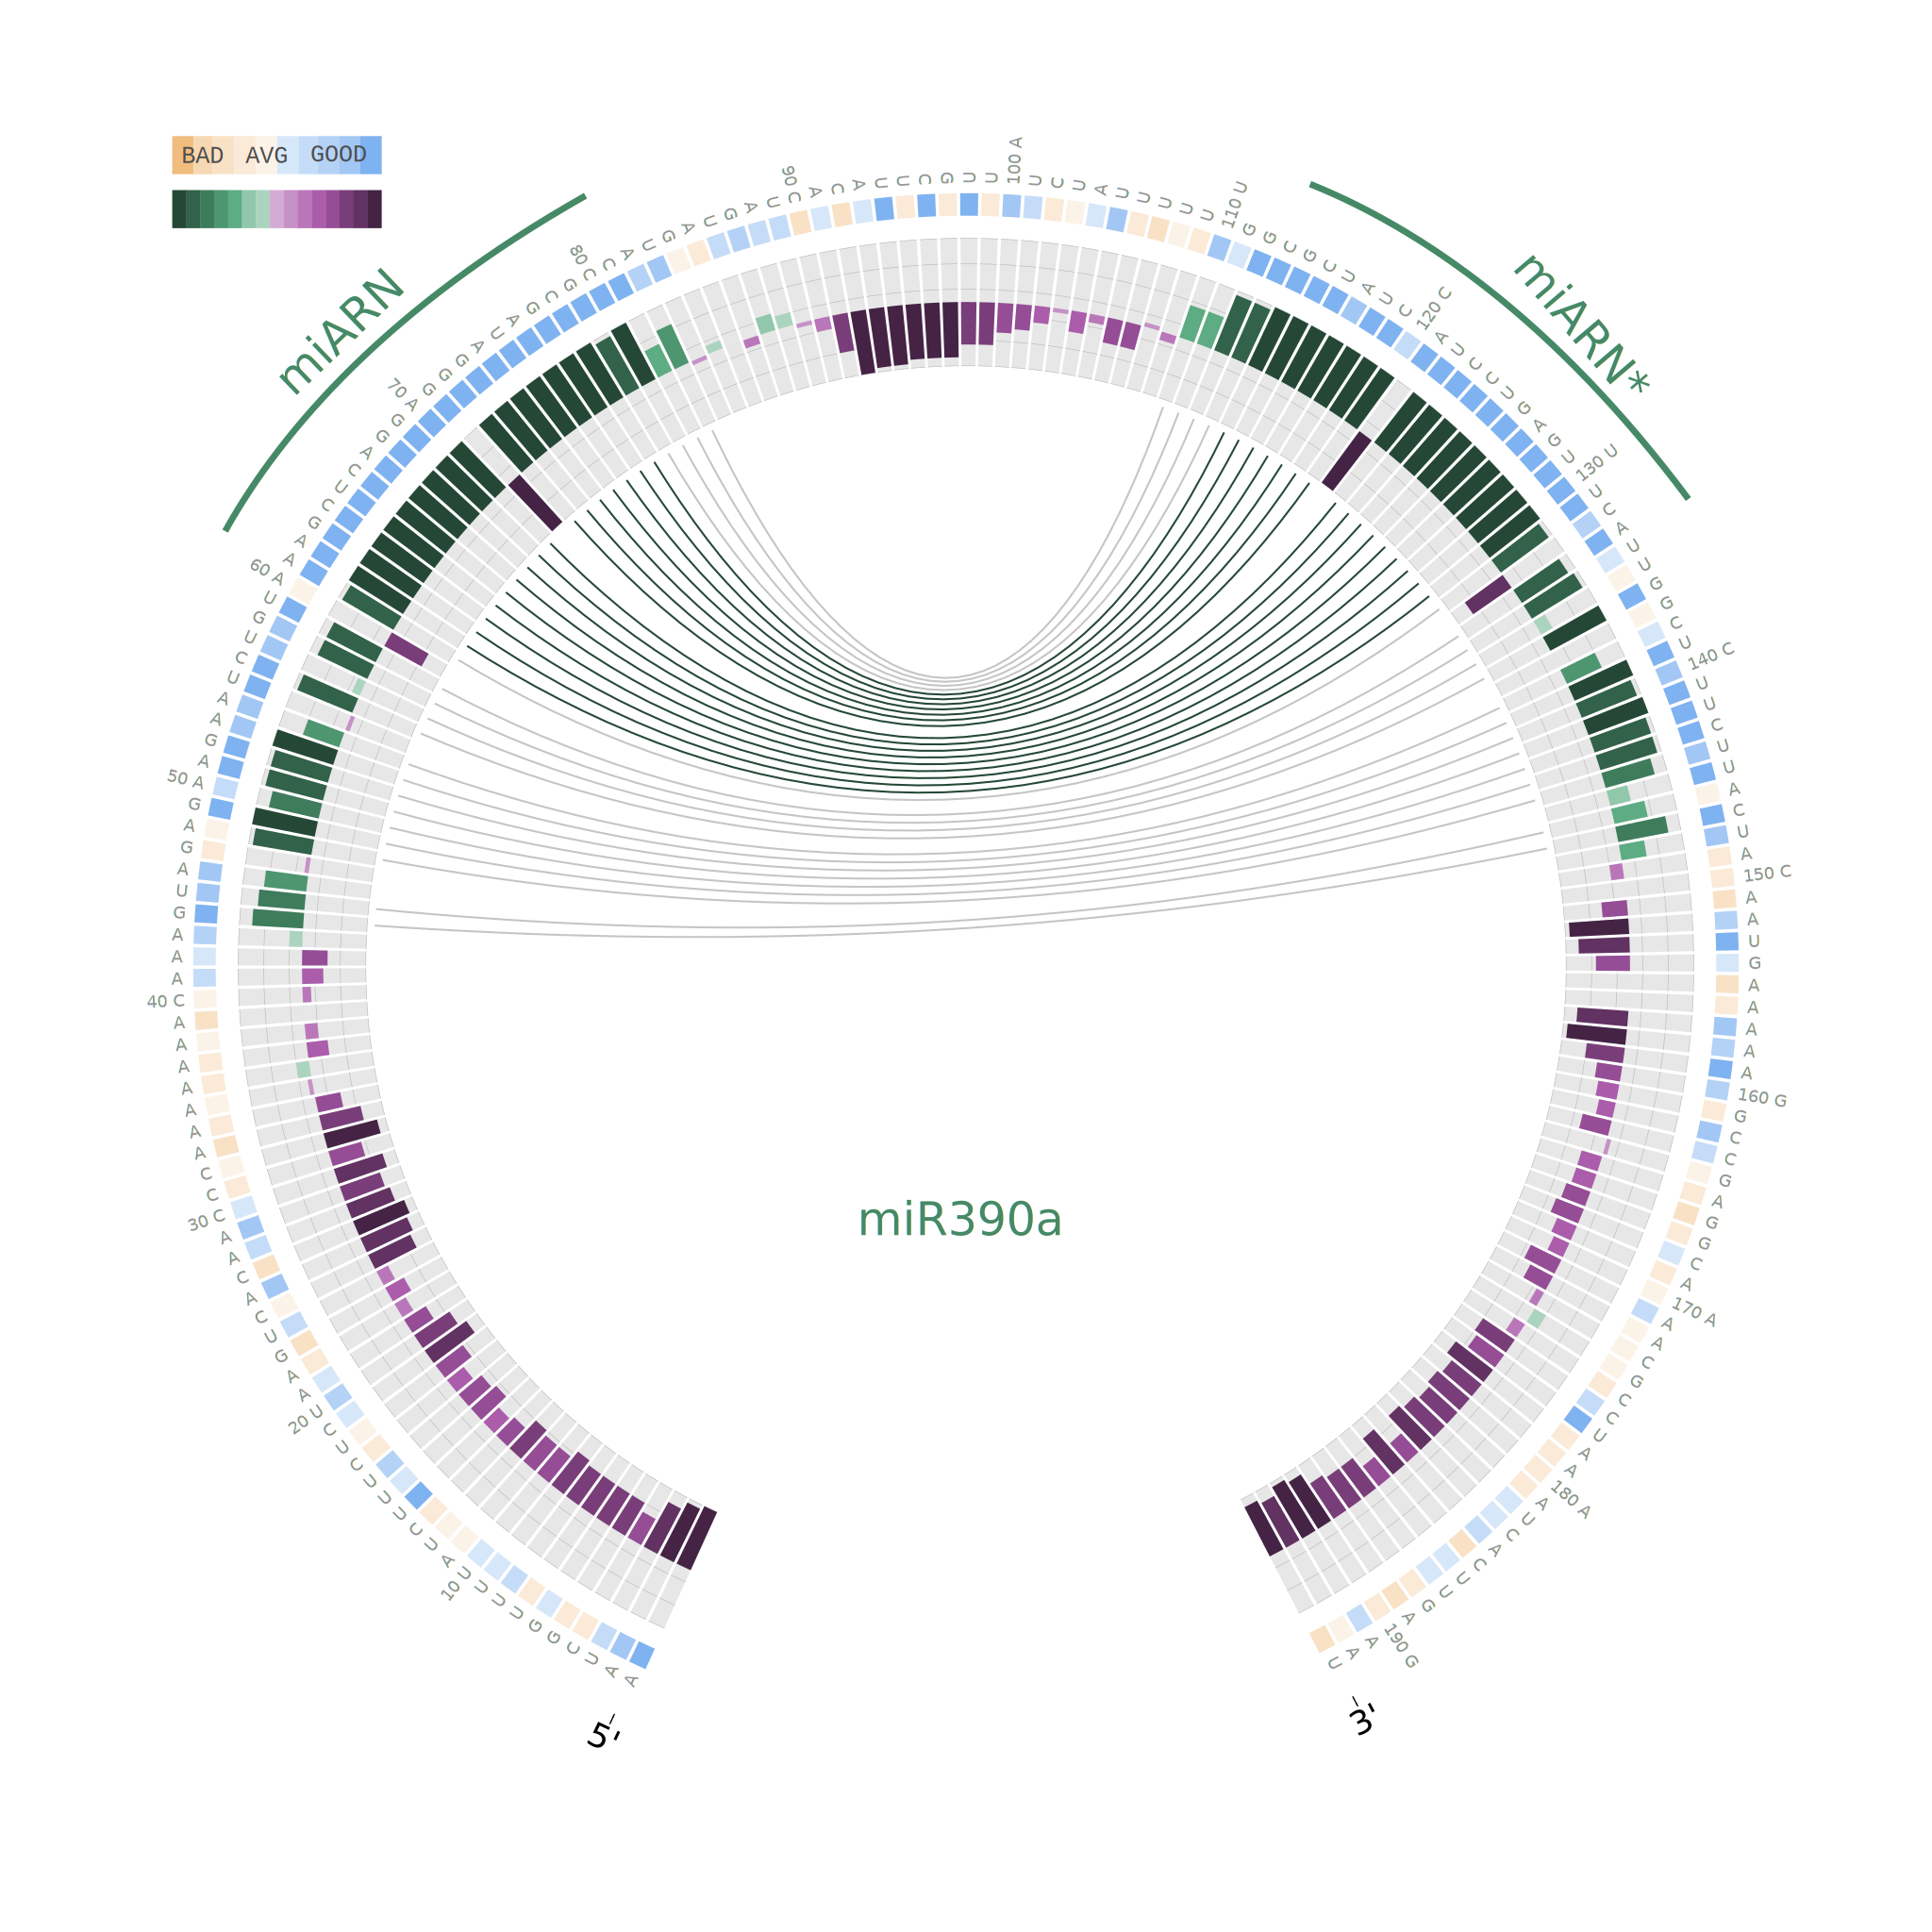
\includegraphics[width=1\textwidth]{miR390a_circos.png}
    \caption[Circos del miR172a]{Circos del miR390a.}
     \label{fig:miR390a_circos}
\end{figure}

\subsubsection{Mecanismo de base a loop secuenciales}

En estos precursores, con un mecanismo secuencial de base a loop, el primer corte procede como en los cortos de base a loop, pero luego son necesario dos cortes más para liberar el miARN, generando en el proceso niveles bajos de RNA pequeños adicionales \citep{Bologna2013}.
Este es el caso de algunos miembros de la  familias del miR169, que tiene en total 14 miembros siendo la familia más grande de \textit{A. thaliana}.
Un estudio en detalle de los precursores del miR169b/d/e/f/g mostró que los sitios de cortes del precursor estaban localizados 21 nt por debajo del lado proximal del dúplex miARN/miARN*.
Esta es la distancia esperada entre dos cortes de DCL1, sugeriendo que estos precursores eran procesados por más de dos cortes de la encima \citep{Bologna2013}.

La familia del miR394 también es procesada de la misma manera y comparten similares patrones de estructura secundaria, donde se ve el tallo inferior largo bien estructurado (Figura \ref{fig:seqBTL_circos}).
Si observamos el patrón de conservación de secuencia primaria podemos ver que la región del dúplex miARN/miARN está muy conservada, pero además podemos observar que debajo del dúplex existe otra región conservada que coincide con el tallo inferior largo que presentan estos precursores (Figura \ref{fig:seqBTL_circos}).

%~ 394b 26 especies
%~ 319b 22 especies

\begin{landscape}
	\begin{figure}
	\centering
	\begin{subfigure}{.75\textwidth}
	  \centering
	  \includegraphics[width=.9\linewidth]{miR169b_circos.png}
	  \caption{Precursor del miR169b}
	  \label{subfig:miR169b_circos}
	\end{subfigure}%
	\begin{subfigure}{.75\textwidth}
	  \centering
	  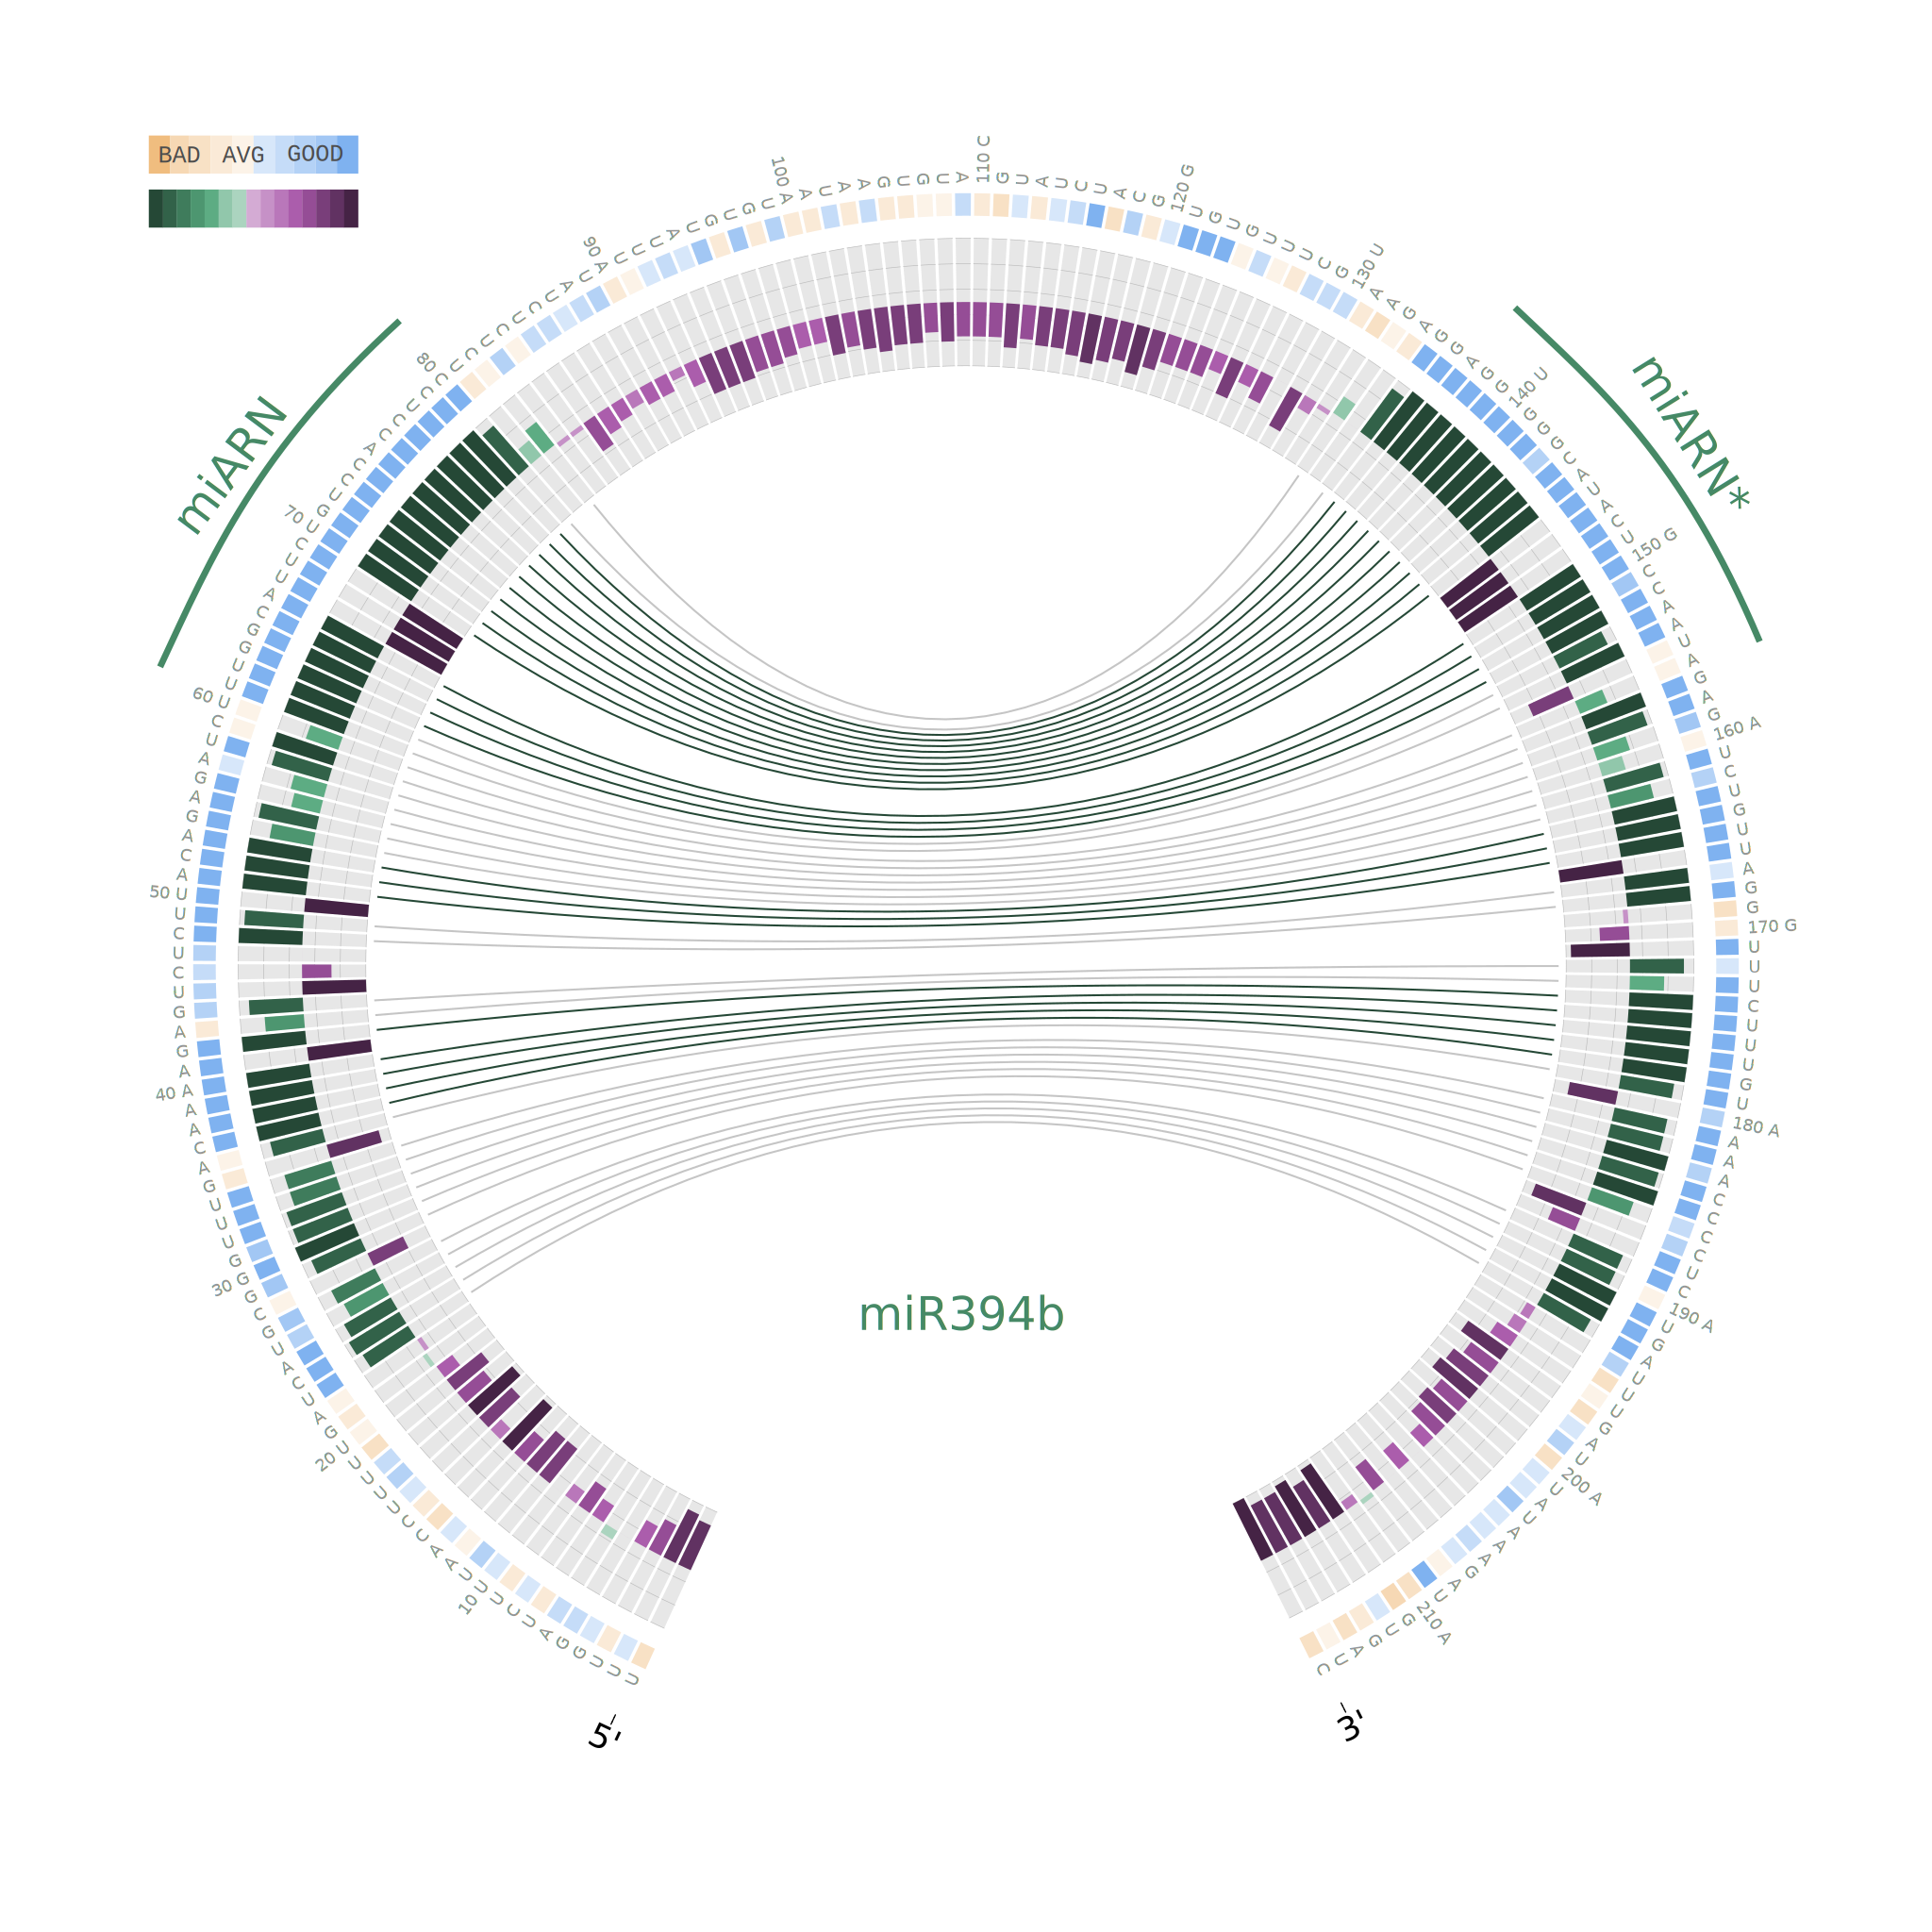
\includegraphics[width=.9\linewidth]{miR394b_circos.png}
	  \caption{Precursor del miR394b}
	  \label{subfig:miR394b_circos}
	\end{subfigure}
	\caption{Circos de precursores con mecanismos de procesamientos secuenciales de base a loop}
	\label{fig:seqBTL_circos}
	\end{figure}
\end{landscape}


\subsubsection{Mecanismo de loop a base cortos}

En los precursores con un mecanismo \textbf{cortos de loop a base}, el procesamiento es guiado por un tallo superior, y son necesarios dos cortes para liberar el miARN maduro.
La región terminal de estos precursores tienen una largo conservado de $\sim$42, donde incluye un loop pequeño \citep{Bologna2013} a diferencia de los precursores procesados dee base a loop, donde esta región es variable en tamaño.

En este caso mostramos los Circos para el precursor del miR157a, que fue encontrado en 30 especies, y para el precursor del miR160a también encontrado en 30 especies. 
En los precursores que se procesan cortos de base a loop observamos que presentan una región conservada que corresponde al tallo superior además de la región que comprende al dúplex miARN/miARN* (Figura \ref{fig:seqBTL_circos}).
A diferencia de los precursores que se procesan de la base al loop, estos precursores no presentan el tallo inferior ni estructurado ni conservado y esto se puede observar en ambos casos; en el miR157a (Figura \ref{subfig:miR157a_circos}) y del miR160a (Figura \ref{subfig:miR160a_circos}).


\begin{landscape}
	\begin{figure}
	\centering
	\begin{subfigure}{.75\textwidth}
	  \centering
	  \includegraphics[width=.9\linewidth]{miR157a_circos.png}
	  \caption{Precursor del miR157a}
	  \label{subfig:miR157a_circos}
	\end{subfigure}%
	\begin{subfigure}{.75\textwidth}
	  \centering
	  \includegraphics[width=.9\linewidth]{miR160a_circos.png}
	  \caption{Precursor del miR160a}
	  \label{subfig:miR160a_circos}
	\end{subfigure}
	\caption{Circos de precursores con mecanismos de procesamientos cortos de loop a base}
	\label{fig:srLTB_circos}
	\end{figure}
\end{landscape}

\subsubsection{Mecanismo de loop a base secuenciales}

En los precursores con un mecanismo \textbf{secuencial de loop a base}, cuatro cortes secuenciales por DCL1 son los encargados de procesar los precursores de miARNs.
En general, estos precursores muestran un tallo largo superior, del cual otros ARNs pequeños son generados \citep{pmid19850910,Bologna2009,Bologna2013}.

En este caso estudiamos la familia del miR319 y del miR159 y en particular mostramos al miR319a (Figura \ref{subfig:miR319a_circos}) y al miR159b (Figura \ref{subfig:miR159b_circos}).
Pudimos reconocer el tallo superior conservado y estructurado.
Además se pudo observar que los ARNs pequeños, que se originan del procesamiento de estos precursores, están conservados de la misma manera que el miARN y el miARN* (Figura \ref{fig:seqLTBL_circos}).

\begin{landscape}
	\begin{figure}
	\centering
	\begin{subfigure}{.75\textwidth}
	  \centering
	  \includegraphics[width=.9\linewidth]{miR319a_circos.png}
	  \caption{Precursor del miR319a}
	  \label{subfig:miR319a_circos}
	\end{subfigure}%
	\begin{subfigure}{.75\textwidth}
	  \centering
	  \includegraphics[width=.9\linewidth]{miR159b_circos.png}
	  \caption{Precursor del miR159b}
	  \label{subfig:miR159b_circos}
	\end{subfigure}
	\caption{Circos de precursores con mecanismos de procesamientos secuenciales de loop a base}
	\label{fig:seqLTBL_circos}
	\end{figure}
\end{landscape}


\subsubsection{Procesamiento mixto de miembros de la familia del miR170/miR171}

En general, se sabe que diferentes miembros de una misma familia de miARNs comparten la misma vía de biogenésis. 
Esta observación no sorprende ya que se cree que las familias de miARNs se expanden por eventos de duplicación de un gen ancestral \citep{pmid15565108}.
Sin embargo, ciertos el procesamiento de miembros de ciertas familias pueden variar de uno a otro \citep{Bologna2013}.
Esto sucede, por ejemplo,en la familia del miR171 donde en \textit{A. thaliana} existen 4 miembros. 
El precursor del miR171a es procesado de base a loop, mientras que los precursores del miR171b y miR171c son procesados de loop a base.

Nos pusimos a analizar esta familia en detalle para ver si los patrones de conservación y estructura secundaria eran diferentes o no.
Observamos que el miR171a, que es procesado corto de base a loop, tiene un patrón de conservación similar a los precursores procesados de base a loop, donde el tallo inferior es estructurado y conservado (Figura \ref{subfig:miR171a_circos}).
Por el contrario el miR171c, que es procesado corto de loop a base, muestra conservación en el tallo superior, que además es estructurado, y no así el tallo inferior (Figura \ref{subfig:miR171c_circos}).


%~ #######
%~ ##### TENGO QUE REHACER EL MIR171A en el lab
%~ #######

\begin{landscape}
	\begin{figure}
	\centering
	\begin{subfigure}{.65\textwidth}
	  \centering
	  \includegraphics[width=.9\linewidth]{miR171c_circos.png}
	  \caption{Precursor del miR171c. Procesamiento de loop a base. }
	  \label{subfig:miR171c_circos}
	\end{subfigure}
	\begin{subfigure}{.65\textwidth}
	  \centering
	  \includegraphics[width=.9\linewidth]{miR171a_circos.png}
	  \caption{Precursor del miR171a. Procesamiento de base a loop.}
	  \label{subfig:miR171a_circos}
	\end{subfigure}
	\caption{Procesamiento mixto de miembros de la familia del miR170/miR171}
	\label{fig:familia_miR171_circos}
	\end{figure}
\end{landscape}


\subsubsection{Mutaciones puntuales afectan el procesamiento de miARNs en plantas}
%~ Natural Variation in Biogenesis
%~ Efficiency of Individual
%~ Arabidopsis thaliana MicroRNAs

Se ha demostrado recientemente que un polimorfismo de origen natural que ocurre en el gen del miR164a afecta a la forma de la hoja y la arquitectura del vástago en \textit{A. thaliana}, con los efectos de ser modificados por loci adicionales en el genoma \citep{pmid22206705}.
Una sustitución única en un par de bases en la secuencia complementaria del miARN altera la estabilidad predicha del dúplex miARN/miARN*.
Se reduce con ello, en gran medida, la acumulación del miARN maduro, probablemente porque interfiere en el procesamiento del precursor.
Además se demostró en ese mismo artículo que no es una rara excepción y que las cepas naturales de \textit{A. thaliana} albergan decenas de polimorfismos similares que afectan al procesaciemiento de una amplia gama de precusores de miARNs.

Es por esto que nos pusimos a estudiar en detalles al precursor del miR164a.
A nivel de secuencia los alelos de Col-0 y C24 son diferentes sólo por un par de polimorfismos simples.
Uno de ellos afecta a una C en el miARN* que aparea con una G en la posición dos del miARN (nos referimos a esta posición como *2) (Figura \ref{fig:miR164_base_pairing}).

\begin{figure}[htbp!] 
	\centering    
	\includegraphics[width=0.6\textwidth]{miR164_base_pairing.png}
	\caption[Apareamiento de bases en el precursor del miR164a]{
		\textbf{Apareamiento de bases en el precursor del miR164a.}
		El miARN se muestra en rojo y el miARN* en azul.
		En la posición *2, el alelo alternativo C24 se muestra en naranja.
	}
	\label{fig:miR164_base_pairing}
\end{figure}

Se puede ver que el remplazo de una G:C en el miR164$a^{Col-0}$ por un par no canónico G:U en el miR164$a^{C24}$, incrementa ligeramente la energía libre del plegado del precursor que cambia de -41.58 kcal/mol a -39.28 kcal/mol, pero no se modifica la estructura secundaria del miR164a (Figura \ref{fig:miR164_ss}). 

\begin{figure}[htbp!] 
	\centering    
	\includegraphics[width=0.3\textwidth]{miR164_ss.png}
	\caption[Estructura secundaria predicha del precursor del miR164a]{
	\textbf{Estructura secundaria predicha del precursor del miR164a.}
	La barra gris horizontal indica el polimorfismo, un G:C en Col-0 y un G:U en C24.
	Los colores indican probabilidad de pares de bases.
	}
	\label{fig:miR164_ss}
\end{figure}

Realizamos el Circos del miR164a en distintas especies para ver como era la conservación de la base en la posición 2* que hace que el precursor no pueda ser procesado de manera correcta.
Lo que pudimos observar es que dicha posición del miR164a* está conservada en dicotiledóneas y se mantiene sin cambios en todas las especies (Figura \ref{miR164a_circos}).
Además esa base está siempre apareada con la base correspondiente del miARN maduro, formando un G:C (Figura \ref{miR164a_circos} a la derecha)..

También se puede observar que en la secuencia del miR164a* existen mutaciones en distintas bases en distintas especies, pero no en la base que estamos estudiando.
Esto sugiere que esa base en particular es importante para la estabilidad del precursor y su buen procesamiento.

%~ \begin{landscape}
    \begin{figure}[htbp!] 
        \centering    
        \includegraphics[width=1\textwidth]{miR164a_circos.png}
        \caption[Circos del miR164a]{
			\textbf{Circos del miR164a}.
			A la izquierda se representa el Circos del miR164a.
			A la derecha el alineamiento del miR164a en distintas especies. 
			Con una flecha verde se destaca la posición *2 a estudiar, en el Circos y en el alineamiento.
        }
        \label{fig:miR164a_circos}
    \end{figure}
%~ \end{landscape}

En otro trabajó, se estudió un alelo mutante llamado miR394b-1, que tiene un mismatch en el stem inferior del precursor del miR394b \citep{pmid23333352}.
La mutante incrementa dramáticamente la terminación del meristema apical.   
En la figura \ref{fig:miR164_base_pairing} se muestra el apareamiento de bases en el precursor del miR394b y miR394b-1, donde el miARN se muestra en rojo y el miARN* en azul.
Y en naranja se muestra la posición de la mutación del precursor del miR394b-1 donde la G es reemplazada por una A con respecto al miR394b.
En este caso se mostró que los niveles de maduro en el precursor del miR394b-1 se ven fuertemente disminuídos aunque no completamente ausentes \citep{pmid23333352}. 

\begin{figure}[htbp!] 
	\centering    
	\includegraphics[width=0.6\textwidth]{miR394b_base_pairing.png}
	\caption[Apareamiento de bases en el precursor del miR394b]{
		\textbf{Apareamiento de bases en el precursor del miR394b.}
		El miARN se muestra en rojo y el miARN* en azul.
		En naranja se muestra la posición de la mutación G por A en el stem inferior del precursor del miR394b-1.
	}
	\label{fig:miR164_base_pairing}
\end{figure}

Para varios precursores de plantas hemos visto anteriormente que esa región que corresponde al stem inferior es crucial para su procesamiento.
En este caso mostramos el Circos correspondiente al miR394b, para poder visualizar que es lo que sucede con esta mutación puntual fuera del dúplex miARN/miARN* (Figura \ref{fig:miR394b_circos_aliniamientos}).
Vemos, como en el caso del miR164a, está mutación que afecta al procesamiento del precursor y a la acumulación del miARN maduro, está conservada en todas las especies estudiadas.
Esto sugiere que esta base es importante para el procesamiento y que no sólo mutaciones de una base dentro del dúplex miARN/miARN* pueden afectar el procesamiento, sino que mutaciones simples en el precursor puede afectar el reconocimiento de DCL1. 

%~ \begin{landscape}
\begin{figure}[htbp!] 
	\centering    
	\includegraphics[width=1\textwidth]{miR394b_circos_aliniamientos.png}
	\caption[Circos del miR394b]{
		\textbf{Circos del miR394b}.
		A la izquierda se representa el Circos del miR394b.
		A la derecha el alineamiento del miR394b en distintas especies. 
		Con una flecha verde se destaca la posición a estudiar, en el Circos y en el alineamiento.
	}
	\label{fig:miR394b_circos_aliniamientos}
\end{figure}
%~ \end{landscape}

%~ Por otro lado, se seleccionaron todos los precursores que codifican para miARNs de la misma familia y luego los analizamos en conjunto.

%~ \subsubsection{Procesamiento central?????}
%~ miR166b 
%~ \subsubsection{Compensatory mutation}
%~ miR164a
%~ miR394b

\subsubsection{Precursores en plantas monocotiledóneas}


\subsubsection{Precursores de animales}

Para esta parte del trabajo de Tesis, utilizamos genomas de distintos especies de \textit{Metazoa} entre ellos humanos, monos, rana, vaca y pez (Tabla \ref{table:db_metazoa}).
Y estudiamos que sucede con los precursores de miARNs conservados en animales.
Para esto partimos de los precursores de humanos definidos en miRBASE.

\begin{table}[!htbp]
\centering
\small
\caption{Especies de \textit{Metazoa} utilizadas}
\label{table:db_metazoa}
\begin{tabular}{c}
\rowcolor[HTML]{ECF4FF} 
\textbf{Animales}        \\
	Bos taurus               \\
	Canis familiaris         \\
	Equus caballus           \\
	Gallus gallus            \\
	Gorilla gorilla          \\
	Homo sapiens             \\
	Macaca mulatta           \\
	Monodelphis domestica    \\
	Mus musculus             \\
	Ornithorhynchus anatinus \\
	Petromyzon marinus       \\
	Sus scrofa               \\
	Xenopus tropicalis      
\end{tabular}
\end{table}


%~ \lhead{Capítulo 4}
%~ 
\graphicspath{{Chapter4/Figs/}}

\setcounter{chapter}{7}
\chapter*{Capítulo 4} 
\addcontentsline{toc}{chapter}{Capítulo 4}
\setcounter{figure}{0}
\setcounter{section}{0}

{\LARGE Estudio bioinformático sobre ARN pequeños y su actividad en \textit{A. thaliana}.}

\section{Introducción}

En plantas existen distintos tipos de ARNs pequeños con distintos tamaño que varían de 20 a 25 nucleótidos, origen y mecanismo de acción.
Basado en las diferencias en su biogénesis y su modo de acción, los ARN pequeños de plantas con funciones regulatorias en la expresión génica han sido agrupados en cuatro clases diferentes
\begin{itemize}
	\item siARNs 	(small interfering RNAs) que es la clase más abundante. 
	\item miARNs (microRNAs). De 20 a 22 nt de longitud.
	\item ta-siARN (trans-acting siARNs)
	\item nat-siARNs y nat-miARNs (natural antisense siRNAs y miRNAs)
\end{itemize}

\section{Resultados y Discusión}

\subsection{Pipeline automatizado para el análisis genómico de ARN pqueños y su actividad in vivo en plantas}

\begin{table}[!htbp]
\centering
\small
\caption{Bibliotecas de ARN pequeños}
\label{my-label}
\begin{tabular}{clcccc}
\rowcolor[HTML]{ECF4FF} 
\hline
Código       & \multicolumn{1}{c}{Muestras de plantas}    & Secuencias totales & \begin{tabular}[c]{@{}c@{}}Lecturas que\\ mapean contra\\ el genoma\end{tabular} & \begin{tabular}[c]{@{}c@{}}Lecturas únicas\\ que mapean\\ contra el genoma\end{tabular} & t/r/sn/snoRNA \\ \hline
col\_8c\_1s  & Muestra 1 a 8°C   & 26594034           & 15235935                                                                         & 2181244                                                                                 & 7933811       \\ \hline
col\_8c\_2s  & Muestra 2 a 8°C   & 24503495           & 14064726                                                                         & 2073756                                                                                 & 7191654       \\ \hline
col\_22c\_1s & Muestra 1 a 22°C  & 13922338           & 6805121                                                                          & 952466                                                                                  & 5420744       \\ \hline
col\_22c\_2s & Muestra 2 a 22°C  & 23037685           & 12430935                                                                         & 1699845                                                                                 & 7575147       \\ \hline
col\_37c\_1s & Muestra 1 a 37°C  & 22273823           & 9109248                                                                          & 1388169                                                                                 & 10127406      \\ \hline
col\_37c\_2s & Muestra 2 a 37°C  & 24307772           & 12748308                                                                         & 1867528                                                                                 & 8511721       \\ \hline
\end{tabular}
\end{table}


Estudiar si se modifica la biogénesis y actividad de los small RNAs en distintas temperaturas.


\begin{figure}[htbp!] 
    \centering    
    \includegraphics[width=1\textwidth]{cantidad_lecturas.png}
    \caption[]{
    \textbf{}
   }
     \label{fig:secuencias_unicas}
\end{figure}


\begin{figure}[htbp!] 
    \centering    
    \includegraphics[width=1\textwidth]{cantidad_lecturas.png}
    \caption[]{
    \textbf{}
   }
     \label{fig:secuencias_unicas}
\end{figure}


\begin{figure}[htbp!] 
    \centering    
    
\includegraphics[width=.5\textwidth]{sRNA_strategy.png}
    \caption[]{
    \textbf{}
   }
     \label{fig:sRNA_strategy}
\end{figure}





\subsection{Biogénesis y actividad de ARN pequeños de plantas en distintas temperaturas}



\lhead{Conclusiones finales}
\setcounter{chapter}{8}
\chapter*{Conclusiones} 
\addcontentsline{toc}{chapter}{Conclusiones}
\setcounter{figure}{0}
\setcounter{section}{0}


\graphicspath{{Chapter2/Figs/}}


\section{Aplicaciones bioinformáticas para el estudio de interacciones miARN-gen blanco}

En cuanto a la primera parte de la Tesis y mediante diferentes estrategias y estudios, hemos alcanzado las siguientes conclusiones:

\begin{itemize}
    \item Diseñamos una estrategia para identificar genes blanco regulados por miARNs en plantas, basado en la conservación evolutiva del par microARN-gen blanco.
    \item El enfoque requiere que la interacción miARN-gen blanco, pueda ocurrir en el contexto de un conjunto mínimo de parámetros que interactúan en diferentes especies. Pero la secuencia del gen blanco en sí, no necesariamente tiene que estar conservada.
    \item Además, nuestro enfoque permite ajustar el número de especies requeridas como un filtro para realizar la búsqueda con diferentes sensibilidades y relaciones señal/ruido.
    \item Utilizando esta estrategia identificamos y validamos experimentalmente nuevos genes blanco en \textit{A. thaliana}, a pesar de que este sistema ya había sido estudiado en detalles en distintos enfoques genómicos a gran escala (\citep{Allen2005207,JonesRhoades2004787,Addo-quaye2009a,German2008,Rajagopalan2006,Schwab2005517}).
    \item Tres de los nuevos genes blanco validados tienen bulges. Parámetros empíricos usualmente le otorgan una gran penalidad a ellos, que puede llegar a ser el doble que un mismatch regular \citep{JonesRhoades2004787}, 
    sin embargo es probable que genes blancos con bulges asimétricos sean más frecuente de lo que se pensaba previamente en plantas.
    \item El enfoque ofrece una estrategia alternativa a otras predicciones que se basan en parámetros empíricos del par miARN-gen blanco \citep{Allen2005207,JonesRhoades2004787,citeulike:8816489,Fahlgren_chapter}.
    \item Una ventaja de la estrategia presentada es que la interacciones miARN-gen blanco conservadas probablemente participen en procesos biológicos relevantes.
    \item Además, esta estrategia puede ser fácilmente modificada para incorporar datos de otras bibliotecas, y/o para realizar la búsqueda de genes blanco presentes en un grupo específico de especies de plantas.
\end{itemize}

Esta parte del trabajo de Tesis fue publicado en la revista Nucleic Acid Research \citep{Chorostecki05072012} y en la revista Bioinformatics \citep{Chorostecki2014}.

%~ We found that newly validated targets have functions related to those already known
%~ MiR159 regulates MYB transcription factors (33,54,55) and NOZZLE (this work), which are involved in stamen and pollen development(48–50,55).
%~ MiR408 regulates the copper transporter PAA2 (this work) as well as copper-binding proteins (13,23,38,56).
%~ MiR167 regulates ARFs (10,57) and IAR3 (this work), and both of them participate in the control of auxin levels and activity (52,58).
%~ These results confirm the importance of miRNA regulation in plants, further indicating that a miRNA might be regulating different components of a biological pathway.


\section{Estudios genómicos sobre la biogénesis de miARNs}

En la segunda parte de esta Tesis, desarrollamos un enfoque genómico a gran escala para estudiar el procesamiento de miARNs en plantas y determinamos, de esta manera, el mecanismo de procesamiento de la mayoría de los miARNs de \textit{A. thaliana} conservados evolutivamente \citep{Bologna2013}.
Encontramos que los miARNs en plantas pueden ser procesados por cuatro mecanismos, dependientes de la dirección secuencial de la maquinaria de procesamiento y del número de cortes requeridos para liberar el miARN (Figura \ref{fig:mecanismos}) \citep{Bologna2013}.
Precursores procesados en el mismo mecanismo comparten determinantes estructurales, explicando el gran rango de tamaño y forma observado en precursores de miARNs en plantas \citep{Bologna2013}.
Además desarrollamos una estrategia bioinformática y luego una herramienta para estudiar a los intermediarios de procesamiento en plantas mutantes en proteínas de procesamiento.
Con esta herramienta se puede determinar la dirección de procesamiento y se puede observar diferencias en los cortes determinados por DCL1 y precisión de la maquinaria en mutantes de procesamiento.

%~ Por último...
%~ , agrupamos toda esta información en una representación gráfica para poder visualizar de manera más simple los precursores de miARNs. 
%~ Caracterizamos la relación entre patrones de conservación y mecanismos de procesamiento determinados previamente. 
%~ Y pudimos observar que a partir del patrón de conservación se puede deducir el mecanismo de procesamiento de precursores en plantas.



% ********************************** Back Matter *******************************
% Backmatter should be commented out, if you are using appendices after References
%\backmatter

% ********************************** Bibliography ******************************
\begin{spacing}{0.9}

% To use the conventional natbib style referencing
% Bibliography style previews: http://nodonn.tipido.net/bibstyle.php
% Reference styles: http://sites.stat.psu.edu/~surajit/present/bib.htm

\bibliographystyle{apalike}
%\bibliographystyle{plainnat} % use this to have URLs listed in References
%~ \cleardoublepage
\renewcommand\bibname{Bibliografía.}
\lhead{Bibliografía}

\bibliography{References/references} % Path to your References.bib file


% If you would like to use BibLaTeX for your references, pass `custombib' as
% an option in the document class. The location of 'reference.bib' should be
% specified in the preamble.tex file in the custombib section.
% Comment out the lines related to natbib above and uncomment the following line.

%\printbibliography[heading=bibintoc, title={References}]


\end{spacing}


% *************************************** Index ********************************
\printthesisindex % If index is present

%~ \cleardoublepage

%~ \setlength{\voffset}{.35in}
\setlength{\oddsidemargin}{-1cm}


\lhead{Anexo}
% ******************************* Thesis Appendix A ****************************
\setcounter{chapter}{9}
\chapter*{Anexo} 
\addcontentsline{toc}{chapter}{Anexo}
\setcounter{figure}{0}
\setcounter{table}{0}
\setcounter{section}{0}

\graphicspath{{Appendix/Figs/}}

\lstinputlisting[caption={circos.conf},label={circos.conf}]{scripts/circos.conf}

\lstinputlisting[caption={histogram.conf},label={histogram.conf}]{scripts/histogram.conf}

\lstinputlisting[caption={links.conf},label={inks.conf}]{scripts/links.conf}

\setlength{\oddsidemargin}{-1cm}


\begin{landscape}
    \begin{figure}[htbp!] 
        \centering    
        \includegraphics[width=1.4\textwidth]{circos_all_01.png}
        \caption[Circos de dicotiledóneas (en más de 20 especies). 1/5]{
        \textbf{Circos de dicotiledóneas donde se detectan ortólogos en más de 20 especies de las 30 analizadas.}
        Fig 1/5.
        }
        \label{fig:circos_all_01}
    \end{figure}
\end{landscape}

\begin{landscape}
    \begin{figure}[htbp!] 
        \centering    
        \includegraphics[width=1.3\textwidth]{circos_all_02.png}
        \caption[Circos de dicotiledóneas (en más de 20 especies). 2/5]{
        \textbf{Circos de dicotiledóneas donde se detectan ortólogos en más de 20 especies de las 30 analizadas.}
        Fig 2/5.
        }
        \label{fig:circos_all_02}
    \end{figure}
\end{landscape}

\begin{landscape}
    \begin{figure}[htbp!] 
        \centering    
        \includegraphics[width=1.3\textwidth]{circos_all_03.png}
        \caption[Circos de dicotiledóneas (en más de 20 especies). 3/5]{
        \textbf{Circos de dicotiledóneas donde se detectan ortólogos en más de 20 especies de las 30 analizadas.}
        Fig 3/5.
        }
        \label{fig:circos_all_03}
    \end{figure}
\end{landscape}

\begin{landscape}
    \begin{figure}[htbp!] 
        \centering    
        \includegraphics[width=1.3\textwidth]{circos_all_04.png}
        \caption[Circos de dicotiledóneas (en más de 20 especies). 4/5]{
        \textbf{Circos de dicotiledóneas donde se detectan ortólogos en más de 20 especies de las 30 analizadas.}
        Fig 4/5.
        }
        \label{fig:circos_all_04}
    \end{figure}
\end{landscape}

\begin{landscape}
    \begin{figure}[htbp!] 
        \centering    
        \includegraphics[width=1.3\textwidth]{circos_all_05.png}
        \caption[Circos de dicotiledóneas (en más de 20 especies). 5/5]{
        \textbf{Circos de dicotiledóneas donde se detectan ortólogos en más de 20 especies de las 30 analizadas.}
        Fig 5/5.
        }
        \label{fig:circos_all_05}
    \end{figure}
\end{landscape}


\begin{table}[htbp!]
\tiny
\centering
\caption{Genes blanco validados de familias miARNs conservados en plantas}
\label{table:NAR_table_S3}
\begin{tabular}{ccc}
\textbf{microRNA}      & \textbf{Target}       & \textbf{ID}        \\
miR156/miR157 & SPL          & At1g27370 \\
miR156/miR157 & SPL          & At1g53160 \\
miR156/miR157 & SPL          & At2g33810 \\
miR156/miR157 & SPL          & At3g15270 \\
miR156/miR157 & SPL          & At5g43270 \\
miR156/miR157 & SPL          & At1g69170 \\
miR156/miR157 & SPL          & At2g42200 \\
miR156/miR157 & SPL          & At3g57920 \\
miR156/miR157 & SPL          & At5g50670 \\
miR159/miR319 & TCP          & At1g30210 \\
miR159/miR319 & TCP          & At1g53230 \\
miR159/miR319 & TCP          & At2g31070 \\
miR159/miR319 & MYB          & At3g11440 \\
miR159/miR319 & TCP          & At3g15030 \\
miR159/miR319 & TCP          & At4g18390 \\
miR159/miR319 & MYB          & At5g06100 \\
miR159/miR319 & MYB          & At2g26950 \\
miR159/miR319 & MYB          & At2g32460 \\
miR159/miR319 & MYB          & At5g55020 \\
miR160        & ARF          & At1g77850 \\
miR160        & ARF          & At2g28350 \\
miR160        & ARF          & At4g30080 \\
miR162        & DCL          & At1g01040 \\
miR164        & NAC          & At1g56010 \\
miR164        & NAC          & At3g15170 \\
miR164        & NAC          & At5g07680 \\
miR164        & NAC          & At5g53950 \\
miR164        & NAC          & At5g61430 \\
miR164        & NAC          & At3g12977 \\
miR164        & NAC          & At5g39610 \\
miR166/miR165 & HD-ZIPIII    & At1g30490 \\
miR166/miR165 & HD-ZIPIII    & At1g52150 \\
miR166/miR165 & HD-ZIPIII    & At2g34710 \\
miR166/miR165 & HD-ZIPIII    & At5g60690 \\
miR166/miR165 & HD-ZIPIII    & At4g32880 \\
miR167        & ARF          & At1g30330 \\
miR167        & ARF          & At5g37020 \\
miR168        & AGO          & At1g48410 \\
miR169        & HAP2         & At1g17590 \\
miR169        & HAP2         & At1g54160 \\
miR169        & HAP2         & At1g72830 \\
miR169        & HAP2         & At3g05690 \\
miR169        & HAP2         & At3g20910 \\
miR169        & HAP2         & At5g06510 \\
miR170/miR171 & SCL          & At2g45160 \\
miR170/miR171 & SCL          & At3g60630 \\
miR170/miR171 & SCL          & At4g00150 \\
miR172        & AP2          & At2g28550 \\
miR172        & AP2          & At4g36920 \\
miR172        & AP2          & At5g60120 \\
miR172        & AP2          & At5g67180 \\
miR172        & AP2          & At2g39250 \\
miR172        & AP2          & At3g54990 \\
miR390/miR391 & TAS3         & At3g17185 \\
miR390/miR391 & TAS3         & At5g49615 \\
miR390/miR391 & TAS3         & At5g57735 \\
miR393        & TIR1/AFB     & At1g12820 \\
miR393        & bHLH         & At3g23690 \\
miR393        & TIR1/AFB     & At3g26810 \\
miR393        & TIR1/AFB     & At3g62980 \\
miR393        & TIR1/AFB     & At4g03190 \\
miR394        & F-Box        & At1g27340 \\
miR395        & APS          & At3g22890 \\
miR395        & AST          & At5g10180 \\
miR395        & APS          & At5g43780 \\
miR395        & APS          & At4g14680 \\
miR396        & GRF          & At2g22840 \\
miR396        & GRF          & At2g36400 \\
miR396        & GRF          & At2g45480 \\
miR396        & GRF          & At4g24150 \\
miR396        & GRF          & At4g37740 \\
miR396        & GRF          & At5g53660 \\
miR396        & GRF          & At3g52910 \\
miR397        & LAC          & At2g29130 \\
miR397        & LAC          & At2g38080 \\
miR397        & LAC          & At5g60020 \\
miR398        & CSD          & At1g08830 \\
miR398        & CSD          & At2g28190 \\
miR398        & CytC oxidase & At3g15640 \\
miR399        & E2-UBC       & At2g33770 \\
miR399        & E2-UBC       & At2g33770 \\
miR408        & LAC          & At2g30210 \\
mir408        & PLC          & At2g02850 \\
miR827        & SPX          & At1g02860
\end{tabular}
\end{table}

\begin{table}[htbp!]
\tiny
\centering
\caption{Mecanismos de procesamiento de miARNs conservados en \textit{A. thaliana}.}
\label{table:mecanismos}
\begin{tabular}{ll}
\textbf{miARN} & \textbf{Mecanismo}        \\
miR156a        & Corto de loop a base      \\
miR156b        & Corto de loop a base      \\
miR156c        & Corto de loop a base      \\
miR156d        & Corto de loop a base      \\
miR156e        & Corto de loop a base      \\
miR156h        & Corto de loop a base      \\
miR157a        & Corto de loop a base      \\
miR157b        & Corto de loop a base      \\
miR157c        & Corto de loop a base      \\
miR159a        & Secuencial de loop a base \\
miR159b        & Secuencial de loop a base \\
miR160a        & Corto de loop a base      \\
miR160b        & Corto de loop a base      \\
miR160c        & Corto de loop a base      \\
miR162a        & Corto de loop a base      \\
miR164b        & Corto de base a loop      \\
miR164c        & Corto de base a loop      \\
miR165a        & Corto de base a loop      \\
miR165b        & Corto de base a loop      \\
miR166a        & Corto de base a loop      \\
miR166b        & Corto de base a loop      \\
miR166f        & Corto de base a loop      \\
miR167a        & Corto de base a loop      \\
miR167b        & Corto de base a loop      \\
miR167c        & Corto de base a loop      \\
miR167d        & Corto de base a loop      \\
miR168a        & Corto de base a loop      \\
miR168b        & Corto de base a loop      \\
miR169a        & Corto de base a loop      \\
miR169b        & Secuencial de base a loop \\
miR169d        & Secuencial de base a loop \\
miR169e        & Secuencial de base a loop \\
miR169f        & Secuencial de base a loop \\
miR169h        & Secuencial de base a loop \\
miR169i        & Secuencial de base a loop \\
miR169j        & Secuencial de base a loop \\
miR169k        & Secuencial de base a loop \\
miR169l        & Secuencial de base a loop \\
miR169m        & Secuencial de base a loop \\
miR169n        & Secuencial de base a loop \\
miR170         & Corto de base a loop      \\
miR171a        & Corto de base a loop      \\
miR171b        & Corto de loop a base      \\
miR171c        & Corto de loop a base      \\
miR172a        & Corto de base a loop      \\
miR172b        & Corto de base a loop      \\
miR172c        & Corto de base a loop      \\
miR172d        & Corto de base a loop      \\
miR172e        & Corto de base a loop      \\
miR319a        & Secuencial de loop a base \\
miR319b        & Secuencial de loop a base \\
miR319c        & Secuencial de loop a base \\
miR390a        & Corto de base a loop      \\
miR390b        & Corto de base a loop      \\
miR391         & Corto de base a loop      \\
miR393a        & Corto de base a loop      \\
miR393b        & Corto de base a loop      \\
miR394a        & Secuencial de base a loop \\
miR394b        & Secuencial de base a loop \\
miR395a        & Corto de base a loop      \\
miR395b        & Corto de base a loop      \\
miR395c        & Corto de base a loop      \\
miR395d        & Corto de base a loop      \\
miR395f        & Corto de base a loop      \\
miR396a        & Corto de base a loop      \\
miR396b        & Corto de base a loop      \\
miR397a        & Corto de base a loop      \\
miR397b        & Corto de base a loop      \\
miR397c        & Corto de base a loop      \\
miR398b        & Corto de base a loop      \\
miR398c        & Corto de base a loop      \\
miR399a        & Corto de base a loop      \\
miR399b        & Corto de base a loop      \\
miR399c        & Corto de base a loop      \\
miR399d        & Corto de base a loop      \\
miR408         & Corto de base a loop      \\
miR827         & Corto de base a loop     
\end{tabular}
\end{table}



\end{document}
